%%%%%%%%%%%%%%%%%%%%%%%%%%%%%%%%%%%%%%%%%%%%%%%%%%%%%%%%%%%%%%%%%%%%%%%%%%%%%%%%
%% Plantilla de memoria en LaTeX para la ETSIT - Universidad Rey Juan Carlos
%%
%% Por Gregorio Robles <grex arroba gsyc.urjc.es>
%%     Grupo de Sistemas y Comunicaciones
%%     Escuela Técnica Superior de Ingenieros de Telecomunicación
%%     Universidad Rey Juan Carlos
%% (muchas ideas tomadas de Internet, colegas del GSyC, antiguos alumnos...
%%  etc. Muchas gracias a todos)
%%
%% La última versión de esta plantilla está siempre disponible en:
%%     https://github.com/gregoriorobles/plantilla-memoria
%%
%% Para obtener PDF, ejecuta en la shell:
%%   make
%% (las imágenes deben ir en PNG o JPG)

%%%%%%%%%%%%%%%%%%%%%%%%%%%%%%%%%%%%%%%%%%%%%%%%%%%%%%%%%%%%%%%%%%%%%%%%%%%%%%%%

\documentclass[a4paper, 12pt]{book}
%\usepackage[T1]{fontenc}

\usepackage[a4paper, left=2.5cm, right=2.5cm, top=3cm, bottom=3cm]{geometry}
\usepackage{times}
\usepackage[utf8]{inputenc}
\usepackage[spanish]{babel} % Comenta esta línea si tu memoria es en inglés
\usepackage{url}
%\usepackage[dvipdfm]{graphicx}
\usepackage{graphicx}
\usepackage{float}  %% H para posicionar figuras
\usepackage[nottoc, notlot, notlof, notindex]{tocbibind} %% Opciones de índice
\usepackage{latexsym}  %% Logo LaTeX

\title{Virtual reality editor for virtual reality scenes}
\author{Julian A. Perez Muñoz}

\renewcommand{\baselinestretch}{1.5}  %% Interlineado

\begin{document}
\cleardoublepage
\chapter{Desarrollo del proyecto}
\label{chap:Desarrollo del proyecto}
Para poder hablar del desarrollo tenemos que comenzar explicando la metodología scrum~\cite{proyectos} ya que hemos seguido una metodología similiar para la creación de este proyecto.

Está metodología, oficialmente surgió en 1995 presentado por Ken Schwaber y Jeff Sutherland mediante "scrum Development Process". Aunque esta fuera la fecha oficial, este modelo ya se había dejado ver en los años 80.

Scrum es un metodología que está centrada en el desarrollo ágil\footnote{\url{https://es.ryte.com/wiki/Desarrollo_Ágil_de_Software}}  de software, aunque he realizado el proyecto de manera individual esta metodología se suele aplicar de manera colectiva con la participación en equipo con el objetivo de obtener el mejor resultado posible.

En Scrum se pueden diferenciar distintos roles, Scrum Master, Product owner y el equipo. El rol de scrum Master en este caso esta representado por el tutor del proyecto cuya función es facilitar y ayudar a gestionar el trabajo. En este caso el product owner no tiene un papel importante y respecto al equipo está representado por mí, el alumno que realiza este proyecto, y su función es el desarrollo y la entrega de las distintas tareas organizadas en cada sprint.

Sobre los sprint, se tratan de distintos periodos de tiempo en el cual el equipo, en este caso yo, me centro en la realización de las tareas marcadas. Estos sprint se inician con un reunión Scrum Master - equipo en la cual se fijaba unos objetivos y se marcaban los pasos a seguir para la consecución de dichos objetivos. Tras un tiempo trabajando en el sprint se emplaza otra nueva reunión en la cual se comparte la tarea terminada y los problemas que han ido surgiendo durante esta.En esta misma reunión el equipo prepara un version funcional de la aplicación o tarea y se marcan los siguientes pasos, el comienzo de un nuevo sprint. 

Podemos ver más en detalle el proceso en la siguiente imagen:
\begin{figure}[H]
  \centering
  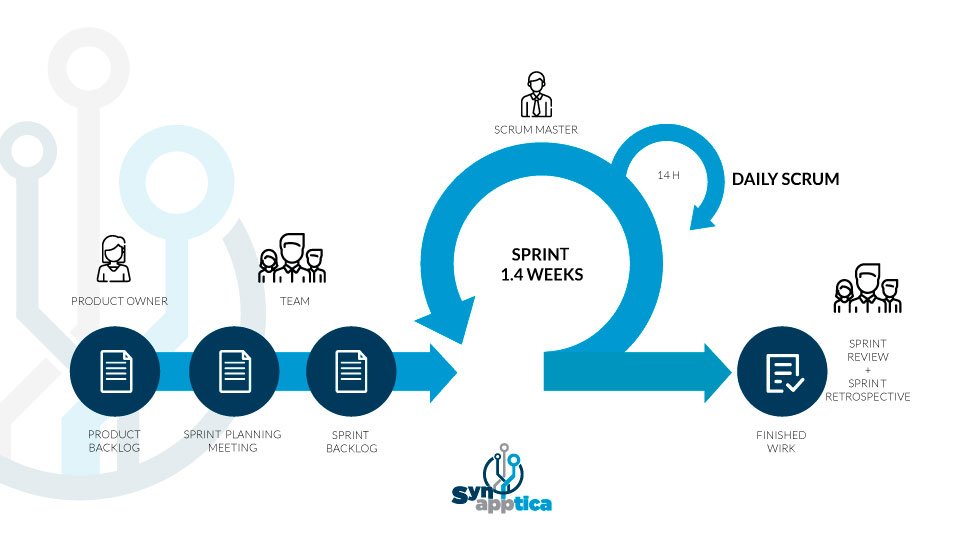
\includegraphics[width=12cm, keepaspectratio]{MemoriaTFG-JulianPerez/img/Scrum.jpg}
  \caption{Estructura metodología Scrum}\label{scrum}
\end{figure}

\section{Sprint 0} % título de sección (se muestra)
\label{sec:sprint0}
En este primer sprint el Scrum Master comenzó a introducir las principales tecnologías que iban a ser usadas en el proyecto, A-frame, JavaScript y HTML. Por lo que en este sprint me dedique a realizar una actividad que asentará la unión entre ambas tecnologías.

\subsection{Objetivo}
El objetivo principal de este Sprint es empezar a usar A-Frame para poder así poder introducrime en la tecnología y aprender como utilizarla. la creación de distintas entidades, eventos, componentes y físicas son los princioales objetivos. En este sprint tenemos que tener en cuenta que una de las principales tecnologías utilizadas, JavaScript, era completamente nueva para mí, por lo que también tuve que aprender sobre esta. Para consolidar todo lo anterior la tarea a realizar fue la creación de un minijuego en el cual crear un componente y que este, reaccionara a un evento.

\subsection{Desarrollo}
Todo comienza haciendose una idea de que va a tratar el minijuego, que componente vamos a crear y que comportamiento le vamos a dar.

Tras pensarlo, concluyo que el minijuego tratará de un recorrido en el cual debes adivinar una de las tres puertas que hay en las diferentes secciones para asi, poder avanzar y llegar al objetivo final del juego.

Para el comportamiento de choque contra la pared, el cual tendrás que realizar para pasar a la siguiente sección utilizaremos el componente Kinema.js que nos proporciona las físicas necesarias para esto. 

El recorrido creado es muy sencillo y presentas las siguientes fases:

\begin{itemize}
    \item Cuando entramos en el juego nos encontramos con la primera sección de tres puertas a adivinar, además, si giramos la cámara nos encontramos con las instrucciones del juego.
    \begin{figure}[H]
  \centering
  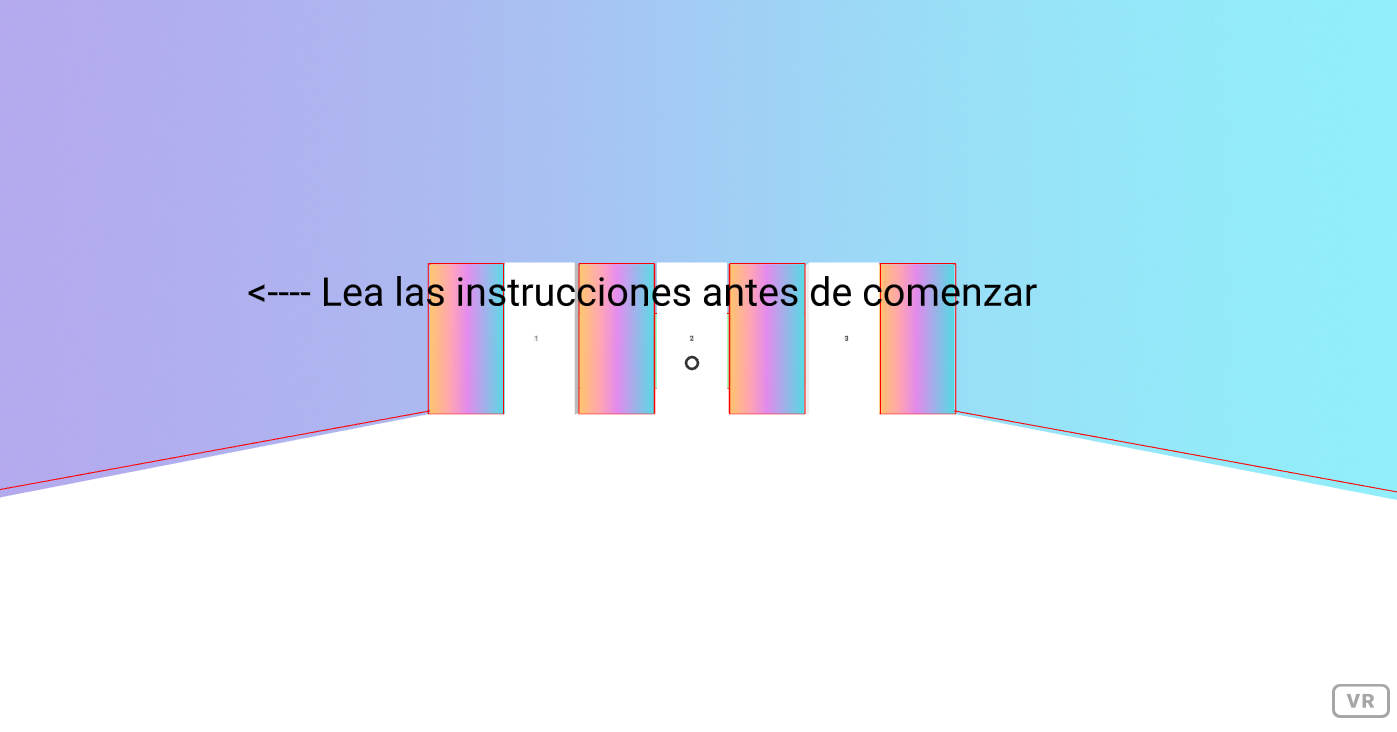
\includegraphics[width=12cm, keepaspectratio]{MemoriaTFG-JulianPerez/img/mini.png}
  \caption{Incio minijuego}\label{scrum}
\end{figure}
    \item Tras esto nos encontramos con tres secciones en las cuales debemos adivinar la puerta para poder avanzar a la siguiente. La manera que tenemos de pasar a la siguiente sección es empujando la puerta, si es la puerta correcta, dicha puerta caerá y podras pasar a la siguiente.
     \begin{figure}[H]
  \centering
  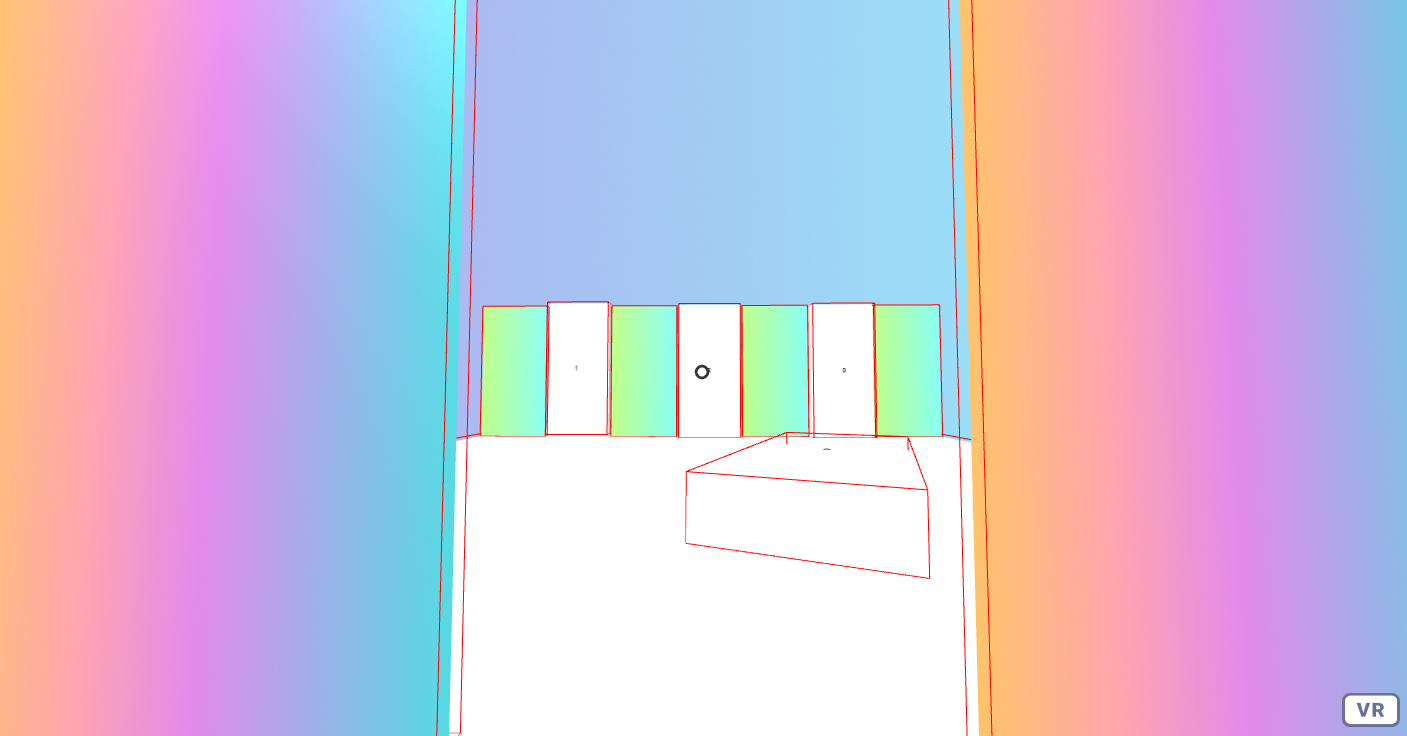
\includegraphics[width=12cm, keepaspectratio]{MemoriaTFG-JulianPerez/img/suelo.png}
  \caption{Situación siguiente sección}\label{scrum}
\end{figure}
    \item Por último tras adivinar todas la puertas, nos encontramos con el objetivo principal del juego, pulsar el botón de la victoria, al cual solo se puede llegar atravesando las puertas. Tras pulsar este botón, el texto que se encuentra en la parte superior te indicará que has ganado.
         \begin{figure}[H]
  \centering
  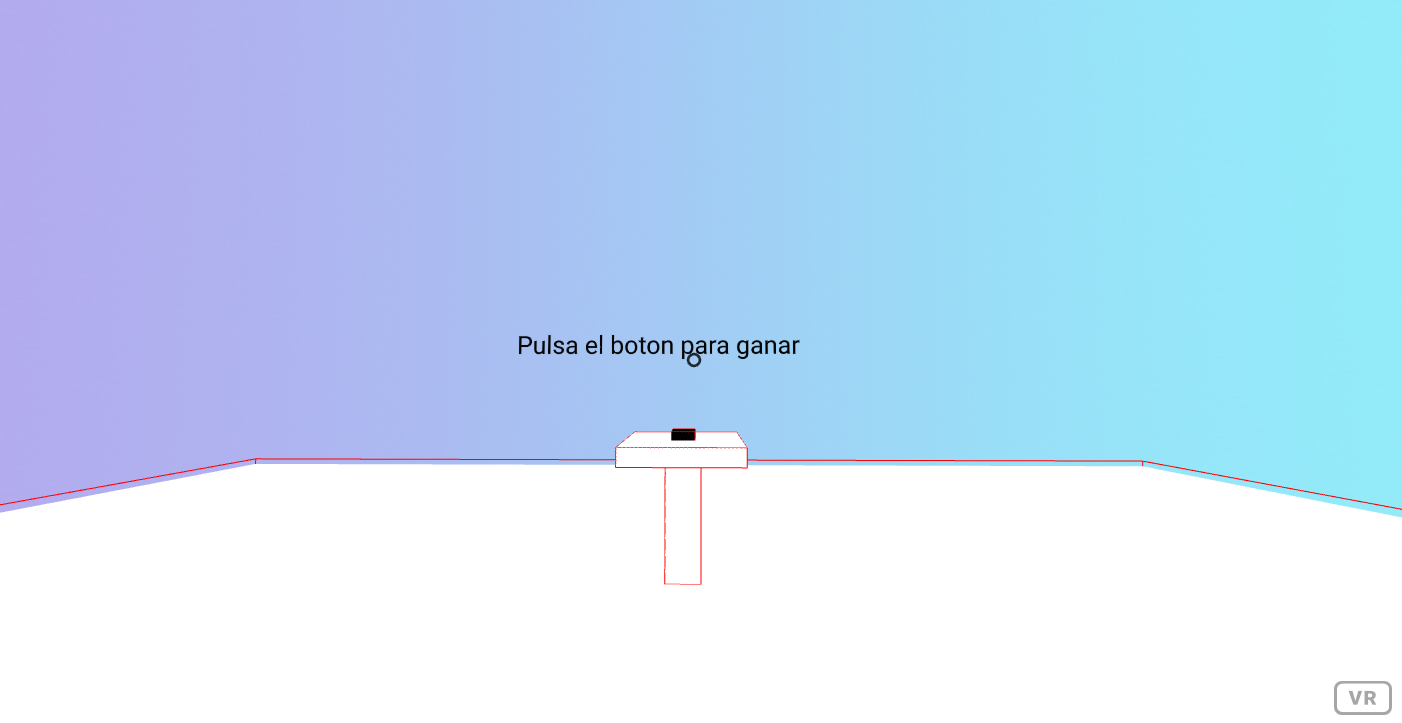
\includegraphics[width=12cm, keepaspectratio]{MemoriaTFG-JulianPerez/img/last.png}
  \caption{Parte final minijuego}\label{scrum}
\end{figure}

\end{itemize}

En cuanto al código creado para este minijuego , cabe destacar lo siguiente:
\begin{verbatim}
<script src="//cdn.rawgit.com/donmccurdy/aframe-physics-system/
v4.0.1/dist/aframe-physics-system.min.js"></script>
<script src="//cdn.rawgit.com/donmccurdy/aframe-extras/
v5.0.0/dist/aframe-extras.min.js"></script>
<script src="components/kinema.js"></script>
\end{verbatim}  
Estas líneas de código localizadas en el elemento \begin{verbatim}
<head>
\end{verbatim} son componentes que nos permiten utilizar distintas funcionalidades que aplicaremos en nuestro minijuego, como puede ser la creación de distintas entidades o la utilización de físicas.

Otra línea de código interesante es:
\begin{verbatim}
<a-box dynamic-body position="0 7.5 15" width="2.3" height="5" 
depth="0.5">
<a-text value="2" color="black" position="-0.1 0 0.5" rotation="0 0 0" 
scale="1 1 1"></a-text>
</a-box>
<a-box static-body position="-5 7.5 15" width="2.3" height="5" 
depth="0.5">
<a-text value="1" color="black" position="-0.1 0 0.5" rotation="0 0 0" 
scale="1 1 1"></a-text>
</a-box>
\end{verbatim} 

Esta parte de código se trata de una parte de la creacíon de las puertas que tienes que elegir, estas, utilizan un componente que proporciona el comportamiento de una entidad fija o movible.\begin{verbatim}dynamic-body/static-body \end{verbatim}

Por útlimo cabe destacar un sencillo componente creado por mí, cuya función es el cambio del texto al pulsar en una entidad.Este texto muestra al usuario que ha conseguido el objetivo del minijuego.  este era realmente el objetivo del sprint la creación de una entidad que reaccionara a un evento.
\begin{verbatim}
AFRAME.registerComponent('nowinnertowinner', {
schema: {
    event: {type: 'string', default: 'click'},
},
init: function () {
    this.eventHandlerClick = function () {
        let text = document.getElementById('WinnerTxt');
        let value = text.getAttribute("value");
        if( value === "Pulsa el boton para ganar"){
            text.setAttribute('value', 'Enhorabuena!!')
            text.setAttribute("scale",{x:3,y:3,z:3});
            text.setAttribute('textwinner', 'Winner');
        }else{
            text.setAttribute('value','Pulsa el boton para ganar')
            text.setAttribute("scale",{x:1,y:1,z:1});
            text.setAttribute('textwinner','noWinner');
        }
    };
},
\end{verbatim} 

         \begin{figure}[H]
  \centering
  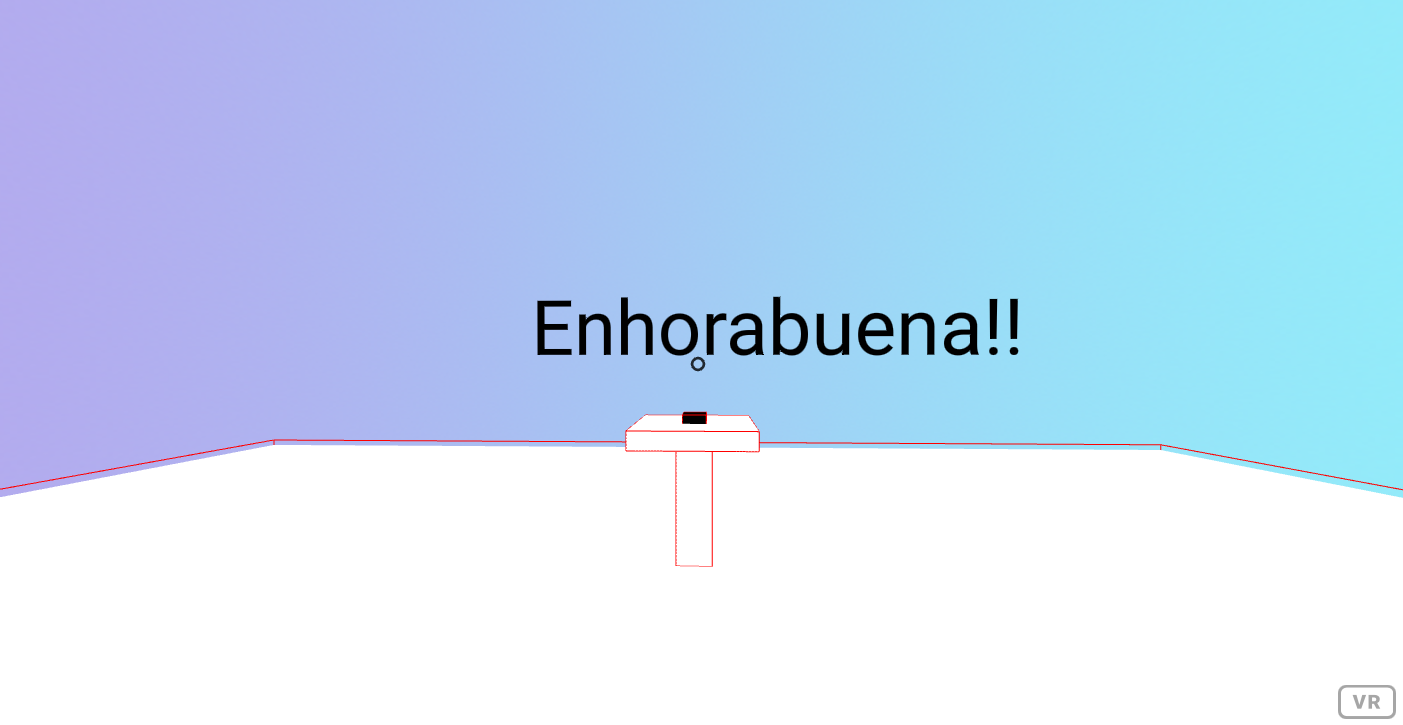
\includegraphics[width=12cm, keepaspectratio]{MemoriaTFG-JulianPerez/img/lastwin.png}
  \caption{Minijuego completado}\label{scrum}
\end{figure}

\subsection{Resultado}
En este primer sprint aprendí las posibilidades que nos puede dar a-frame y a hacerme una idea de como plantear el resto del proyecto, de manera paralela fui aprendiendo a utilizar javascript ya que era una tecnogía no antes usada. Este minijuego se encuentra en el repositorio del proyecto y esta accesible a cualquier persona tanto a la interfaz del juego\footnote{\url{https://julianperezm.github.io/A-frame/FirstExercise/FirstExercise.html}}  como al código\footnote{\url{https://github.com/julianperezm/A-frame/tree/master/FirstExercise}} . Tras esto, se mantuvo la correspondiente reunión con el scrum master en la cual se pone en común lo aprendido y se plantea el siguiente sprint.

\section{Sprint 1}
A partir de este sprint se construirá nuestra aplicación final por lo que podemos decir que este sprint es la base de nuestro proyecto. 
\subsection{Objetivo}
El objetivo de este sprint es la creación de un menú con las cuatro formas básicas de a-frame (plano, cubo, cilindro y esfera). las cuales las podremos seleccionar y apareceran en un lugar determinado de la escena. Para la creacíon de estas acciones utilizaremos tanto elementos HTML como componentes creados en JavaScript.

\subsection{Desarrollo}
Algunos sprints los separaremos en tareas para así organizar mejor este y poder así trabajar lo más eficiente posible. Esto en la metodología scrum, se denomina, bolsa de tareas.

\textbf{Tarea 1}

La primera tratá de simplificar el funcionamiento de lo que queremos en este sprint, por lo que crearemos un botón que crea una figura en la escena. 
Esta primera escena contará con un podium donde aparecera la figura y un botón el cual creará la figura, más adelante ese botón se converitra en las cuatros figuras básicas que al pulsarla mediante el cursor se crean en la escena.
         \begin{figure}[H]
  \centering
  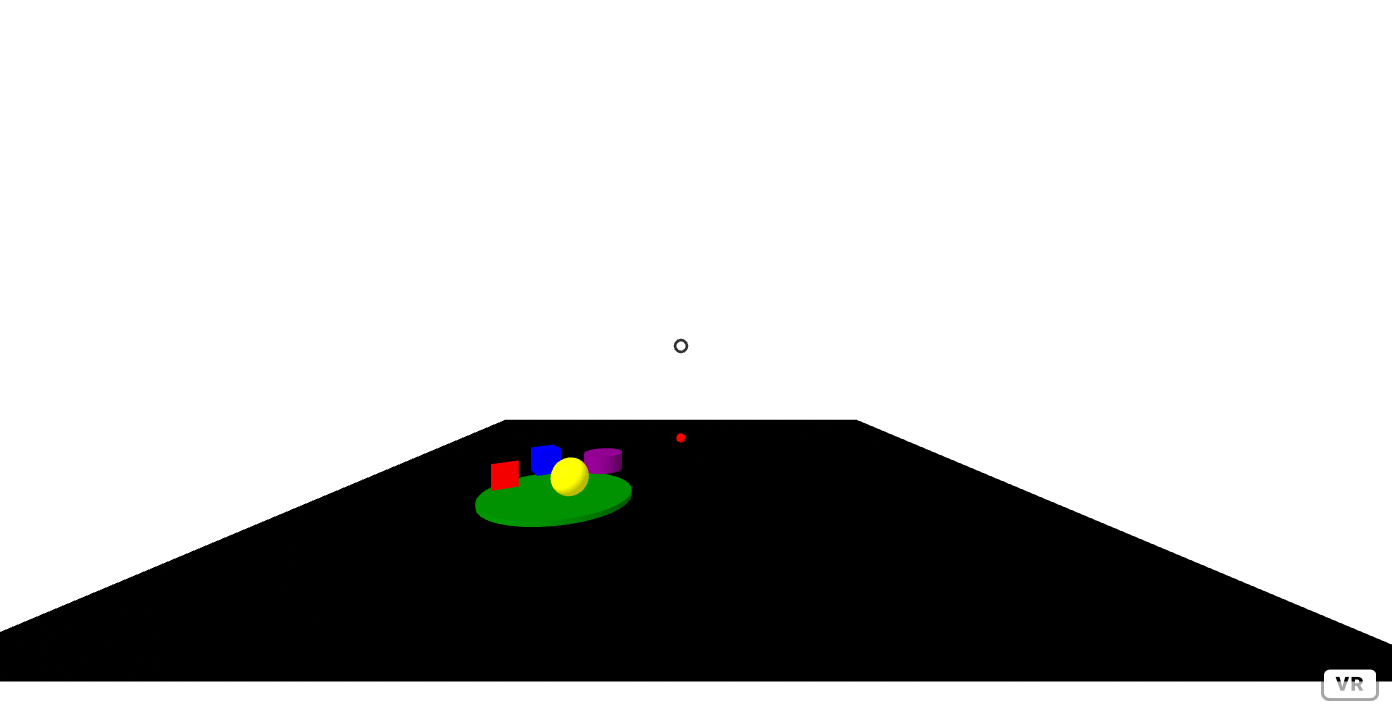
\includegraphics[width=12cm, keepaspectratio]{MemoriaTFG-JulianPerez/img/1.png}
  \caption{Inicio primer ejercicio}\label{scrum}
\end{figure}

\textbf{Tarea 2}

En esta tarea con el fin de crear una interfaz mas amigable y mas funcional, el objetivo era que el menu se moviese para que la figura a la elegir fuera mas accesible. utilizaremos el atributo animación para la creaciópn de la misma.
\begin{verbatim}
 baseMenu.setAttribute('animation', 'property:rotation;to:0 360 0;
 loop:true;dur:10000')   
\end{verbatim}

Tras estas dos tareas de iniciación del proyecto, se tuvo una reunion con el scrum master para saber si se iba por el buen camino, y para terminar de aclarar las siguientes tareas.

\textbf{Tarea 3}

En esta tarea seguimos con la funcionalidad de crear una interfaz mas amigable y pulsar una figura con el cursor de aframe no lo era. Por lo que creamos una interacción con la figura clickando directamente en ellas. A su vez también cambiamos el aspecto del escenario para que fuera mas vistoso al usuario.
         \begin{figure}[H]
  \centering
  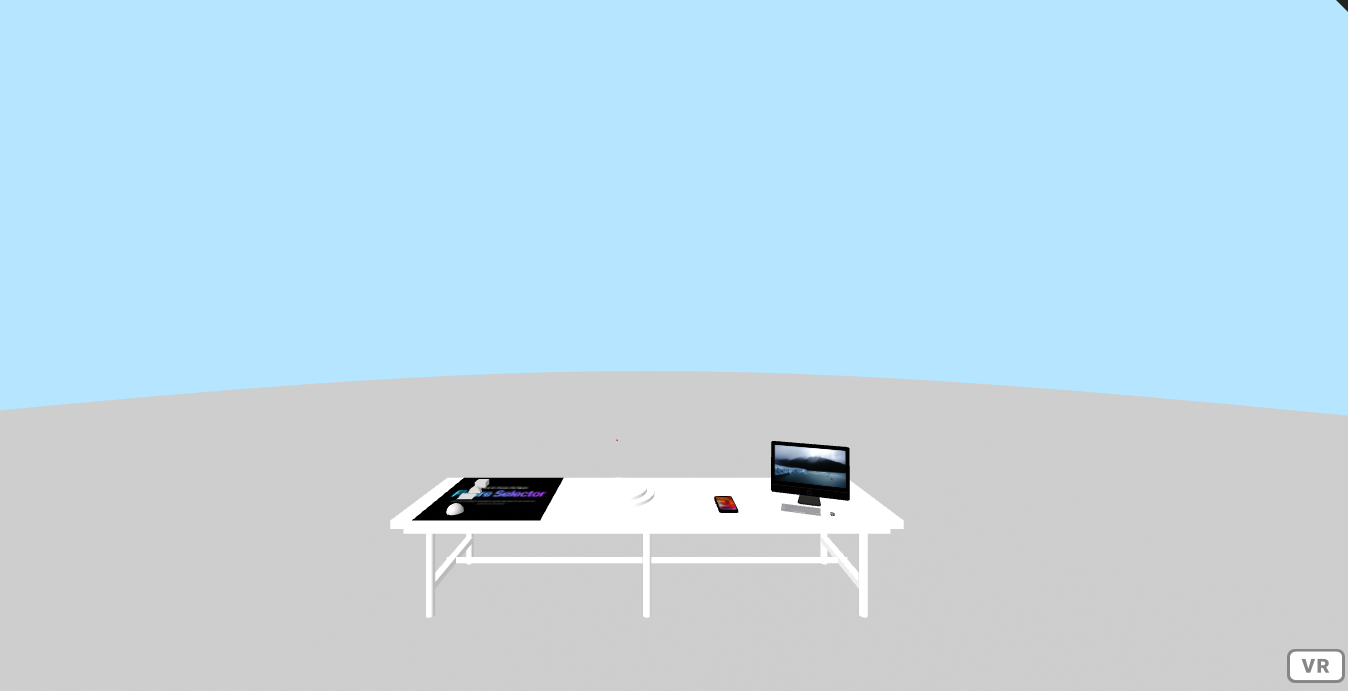
\includegraphics[width=12cm, keepaspectratio]{MemoriaTFG-JulianPerez/img/2.png}
  \caption{Escena inicial con mejora en la interfaz}\label{scrum}
\end{figure}

\textbf{Tarea 4}

Para seguir adelante con la creación del editor, en esta tarea nos centraremos en la funcionalidad, la cual permitirá que las figuras puedan ser arrastradas a cualquier lugar de la escena y que cada una tenga una mini previsualización de distintos colores encima de ella.          \begin{figure}[H]
  \centering
  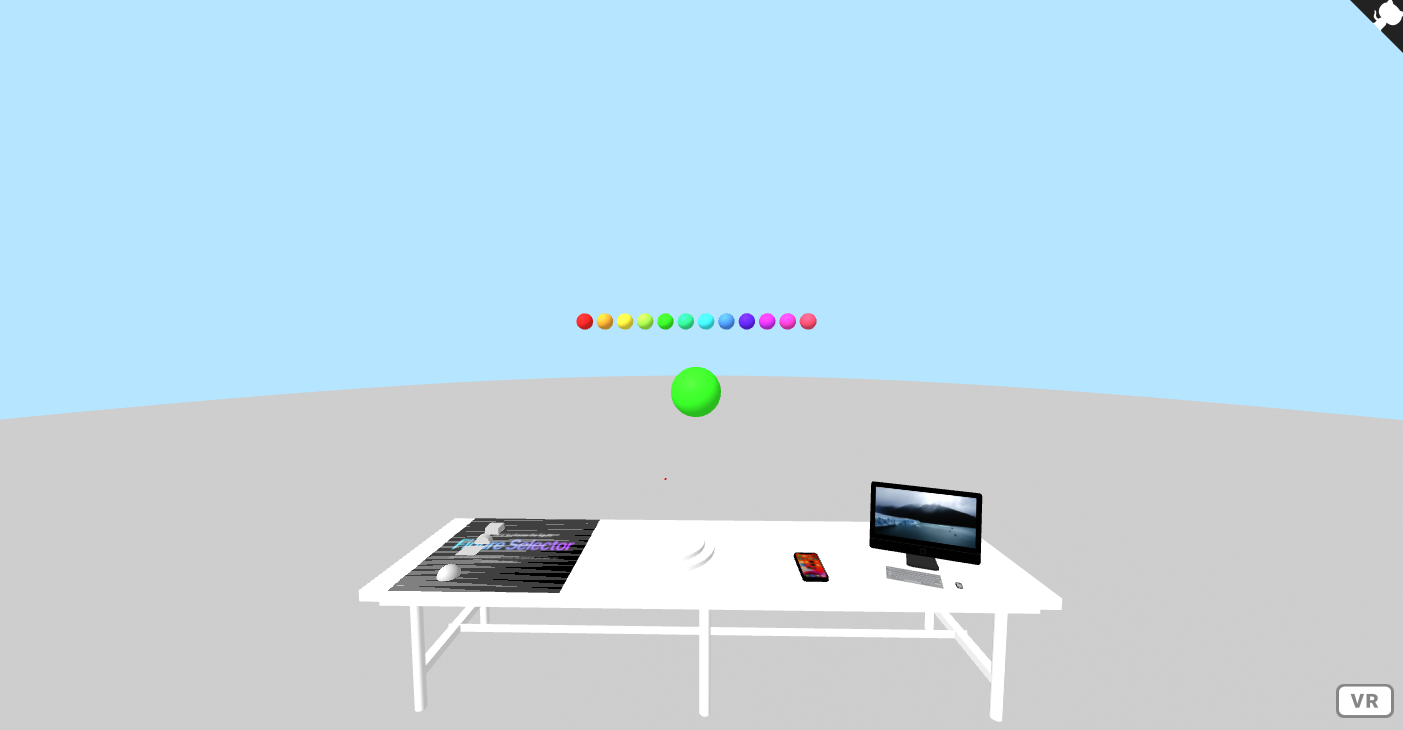
\includegraphics[width=12cm, keepaspectratio]{MemoriaTFG-JulianPerez/img/3.png}
  \caption{Figura creada en la escena}\label{scrum}
\end{figure}

\textbf{Tarea 5}
Por útlimo en esta tarea se empieza a jugar con la creación de modelos en 3d con el formato gltf explicado anteriormente. Insertamos en la escena un dispositivo movil y un ordenador a modo de decoración.
\begin{figure}[H]
  \centering
  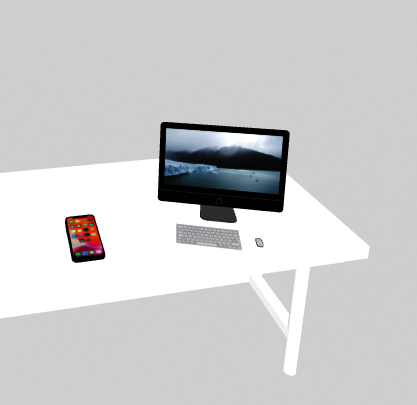
\includegraphics[width=12cm, keepaspectratio]{MemoriaTFG-JulianPerez/img/4.png}
  \caption{Modelos 3D en la escena}\label{scrum}
\end{figure}

\subsection{Resultado}
En este sprint se dio el primera paso de lo que será nuestro editor, hemos creado algunas funcionalidades que nos seran muy utiles en el futuro. Toda esta implentación se encuentra en el repositorio del proyecto en github, esta accesible tanto al codigo \footnote{\url{https://github.com/julianperezm/A-frame/tree/master/ThirdExercise}}
 HTML o JavaScript como a la escena en el navegador\footnote{\url{https://julianperezm.github.io/A-frame/ThirdExercise/ThirdExercise.html}}

\section{Sprint 2}
En este sprint tras haber empezado nuestro proyecto, nos centraremos en las disitntas posibilidades de modificación de propiedades, la creación de distintas  funcionalidades y la mejora de la interfaz de la aplicación.

\subsection{Objetivo}
Nos centraremos en tres objetivos principales, la modificación de una propiedad concreta de las figuras, el tamaño. Nos centraremos también en la creación de una de las funcionalidades principales de la aplicación, la creacíon de un modo grupo de figuras. A la vez que realizamos estos ejercicios nos centraremos en la mejora de la interfaz de la aplicación para que sea mas usable en 3D.

\subsection{Desarrollo}
Como en los casos anteriores separaremos el desarrollo del sprint en diferentes tareas.

\textbf{Tarea 1}

En esta tarea nos centraremos en la creación de la funcionalidad que llamaremos, modo grupo. Esta funcionalidad consiste en la unión de diferentes figuras que seran manejadas por otra figura que llamaremos, manejador. 

Esta funcionalidad es útil por si queremos crear una figura que se base en la unión de varias. Él metodo por el que realizaremos esta funcionalidad es mediante la creación de distintos componentes. La manera de acceder a ella es pulsando la tecla q. 

El resultado de esta tarea se puede observar en un panel creado en el escenario, cuando el modo grupo este activado se mostrará como se puede observar en la figura 3.11, del mismo modo cuando esté activado figura 3.10.

\begin{figure}[H]
  \centering
  \begin{minipage}[b]{0.4\textwidth}
 
\includegraphics[width=7cm]{MemoriaTFG-JulianPerez/img/single.png}
  \caption{Modo grupo desactivado}\label{single}
  \end{minipage}
  \hfill
  \begin{minipage}[b]{0.4\textwidth}
  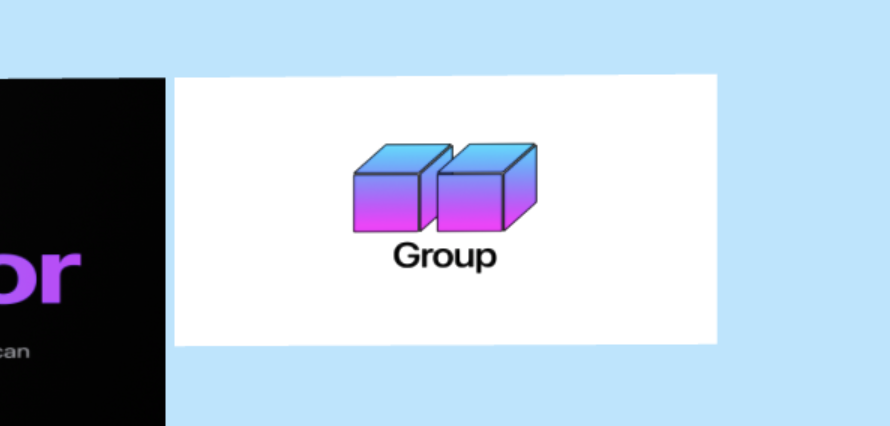
\includegraphics[width=7cm]{MemoriaTFG-JulianPerez/img/group.png}
  \caption{Modo grupo activado}\label{scrum}
  \end{minipage}
\end{figure}

\textbf{Tarea 2}

Tras la creación de la funcionalidad, nos centraremos en la modificación de una de las propiedas de la figura. La modificación se centra en el tamaño, recordemos que anteriormente añadimos el poder cambiar el color de la figura.

Esto lo realizaremos de una manera similiar, crear disitintas componentes que permitan modificar la escala de la figura, con una particularidad, podremos modificar la escala en los distintos ejes para así poder tener más posibilidades a la hora de crear diferentes figuras. 

Esta tareas se puede visualizar en la escena mediante diferentes botones que se pueden ver en la figura 3.12 además de esto, podrás ver las medidas de la figura creada.

\begin{figure}[H]
  \centering
  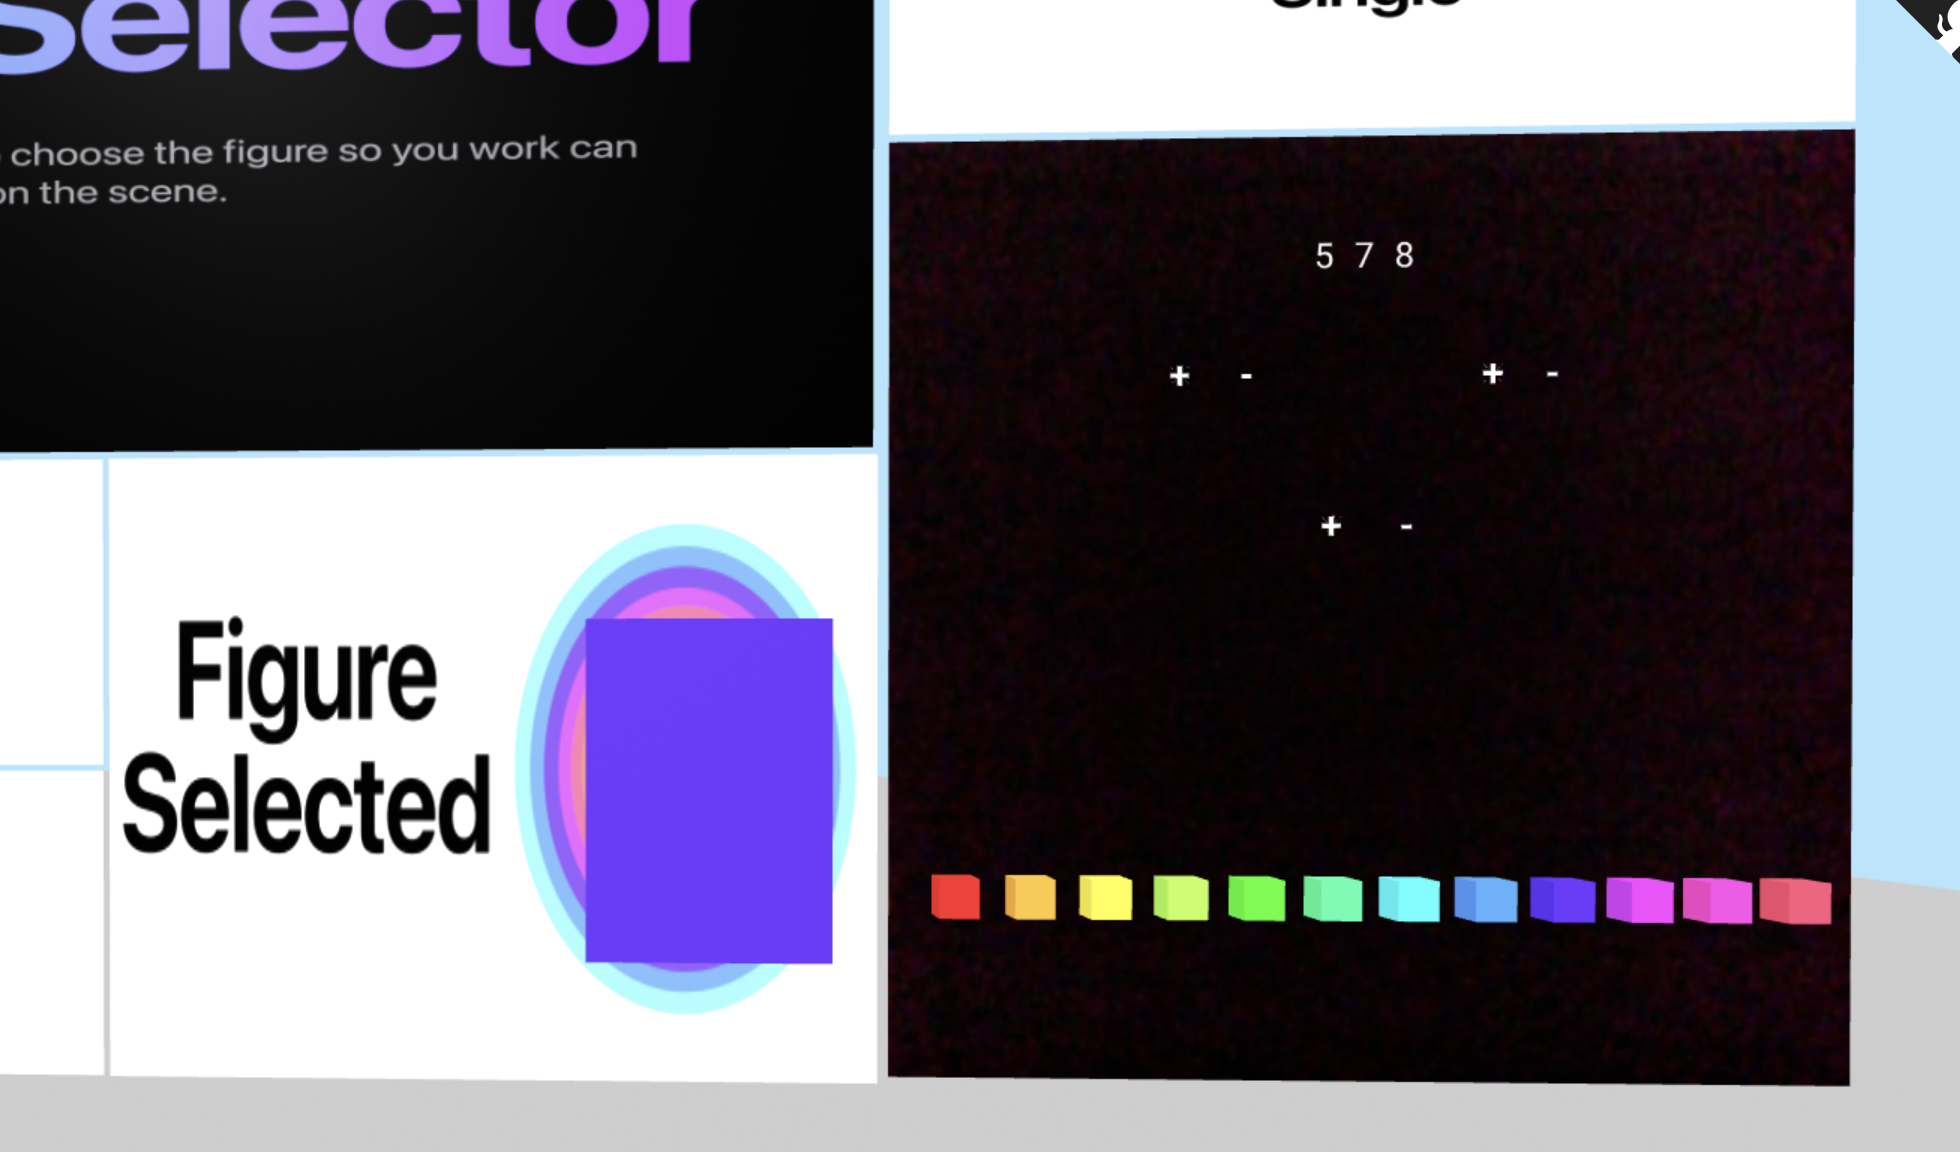
\includegraphics[width=12cm, keepaspectratio]{MemoriaTFG-JulianPerez/img/tam.png}
  \caption{Menú modificación figura}\label{scrum}
\end{figure}


Tras estas dos tareas, se realizó una reunión con el scrum master, donde se le enseñó las tareas realizadas y se puso en común la siguiente tarea a realizar, mejorar el escenario para que tenga una mejor integracíon en 3D y sea más vistoso al usuario.

\textbf{Tarea 3}

En esta tarea nos centraremos en la mejora de la interfaz de la aplicación para que sea más usable y mas vistoasa para el usuario. 

Los paneles de información de la aplicación en vez de ser planos se les dara un poco de profundida, el menu de selección de figuras, pasará a ser en 3D para que sea mas intutivo, y la modificación del tamaño pasa a ser mediente slides para hacerlo mas sencillo.

El resultado se puede observar en la figura 3.13

\begin{figure}[H]
  \centering
  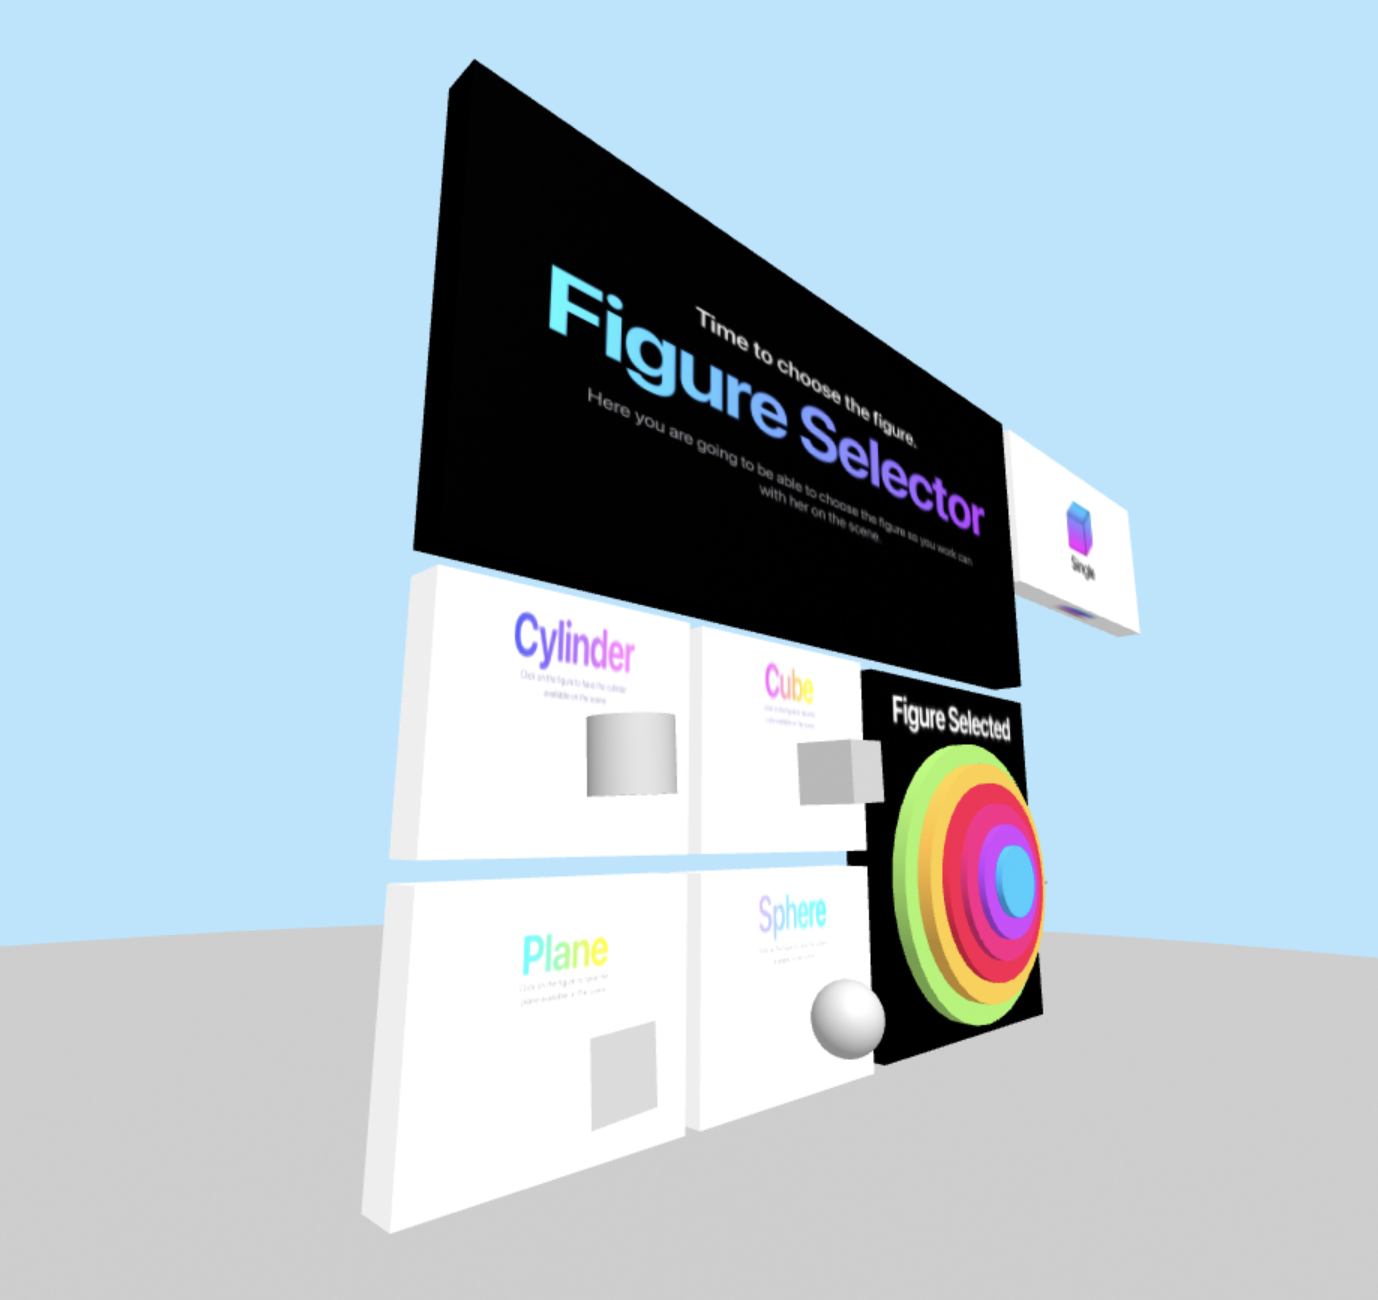
\includegraphics[width=12cm, keepaspectratio]{MemoriaTFG-JulianPerez/img/prof.png}
  \caption{Nueva interfaz de la aplicación}\label{scrum}
\end{figure}

\subsection{Resultados}

En este sprint hemos conseguido mejorar considerablemente nuestro editor, ya que hemos añadido una nueva funcionalidad, hemos añadido un metodo más de modificación de la figura y hemos mejorado el escenario para un uso mas fácil de este. Este sprint está disponible en el repositorio del proyecto en github, tanto el código\footnote{\url{https://github.com/julianperezm/A-frame/tree/master/FifthExerciseV1}} como el escenario \footnote{\url{https://julianperezm.github.io/A-frame/FifthExerciseV1/FifthExercise.html}}


\section{Sprint 3}

En este sprint seguiremos mejorando la interfaz de usuario de la aplicación además de añadirle nuevas funcionalidades como la creación de nuevas figuras con el formato GLTF o seguir añadiendo cambios en las propiedas de las figuras.

\subsection{Objetivo}
Para este sprint tenemos varios objetivos en los que centrarnos, respecto a la mejora de la interfaz me centraré en disitintos puntos como son las dimensiones del escenario y la visibilidad de distintos objetos. Añadiremos la funcionalidad de poder añadir nuevas figuras con el formato gltf y modificar propiedas de estas y haremos nuestra aplicación compatible con las gafas de realidad virtual.

\subsection{Desarrollo}
Las tareas para este sprint son las siguientes:

\textbf{Tarea 1}

En esta tarea nos centraremos en la mejora de la interfaz de usuario. Rediseñaremos el escenario en cuanto al tamaño, ya que el escenario anterior no se adecuaba de manera correcta, ya que las figuras eran demasiado grandes. 

\begin{figure}[H]
  \centering
  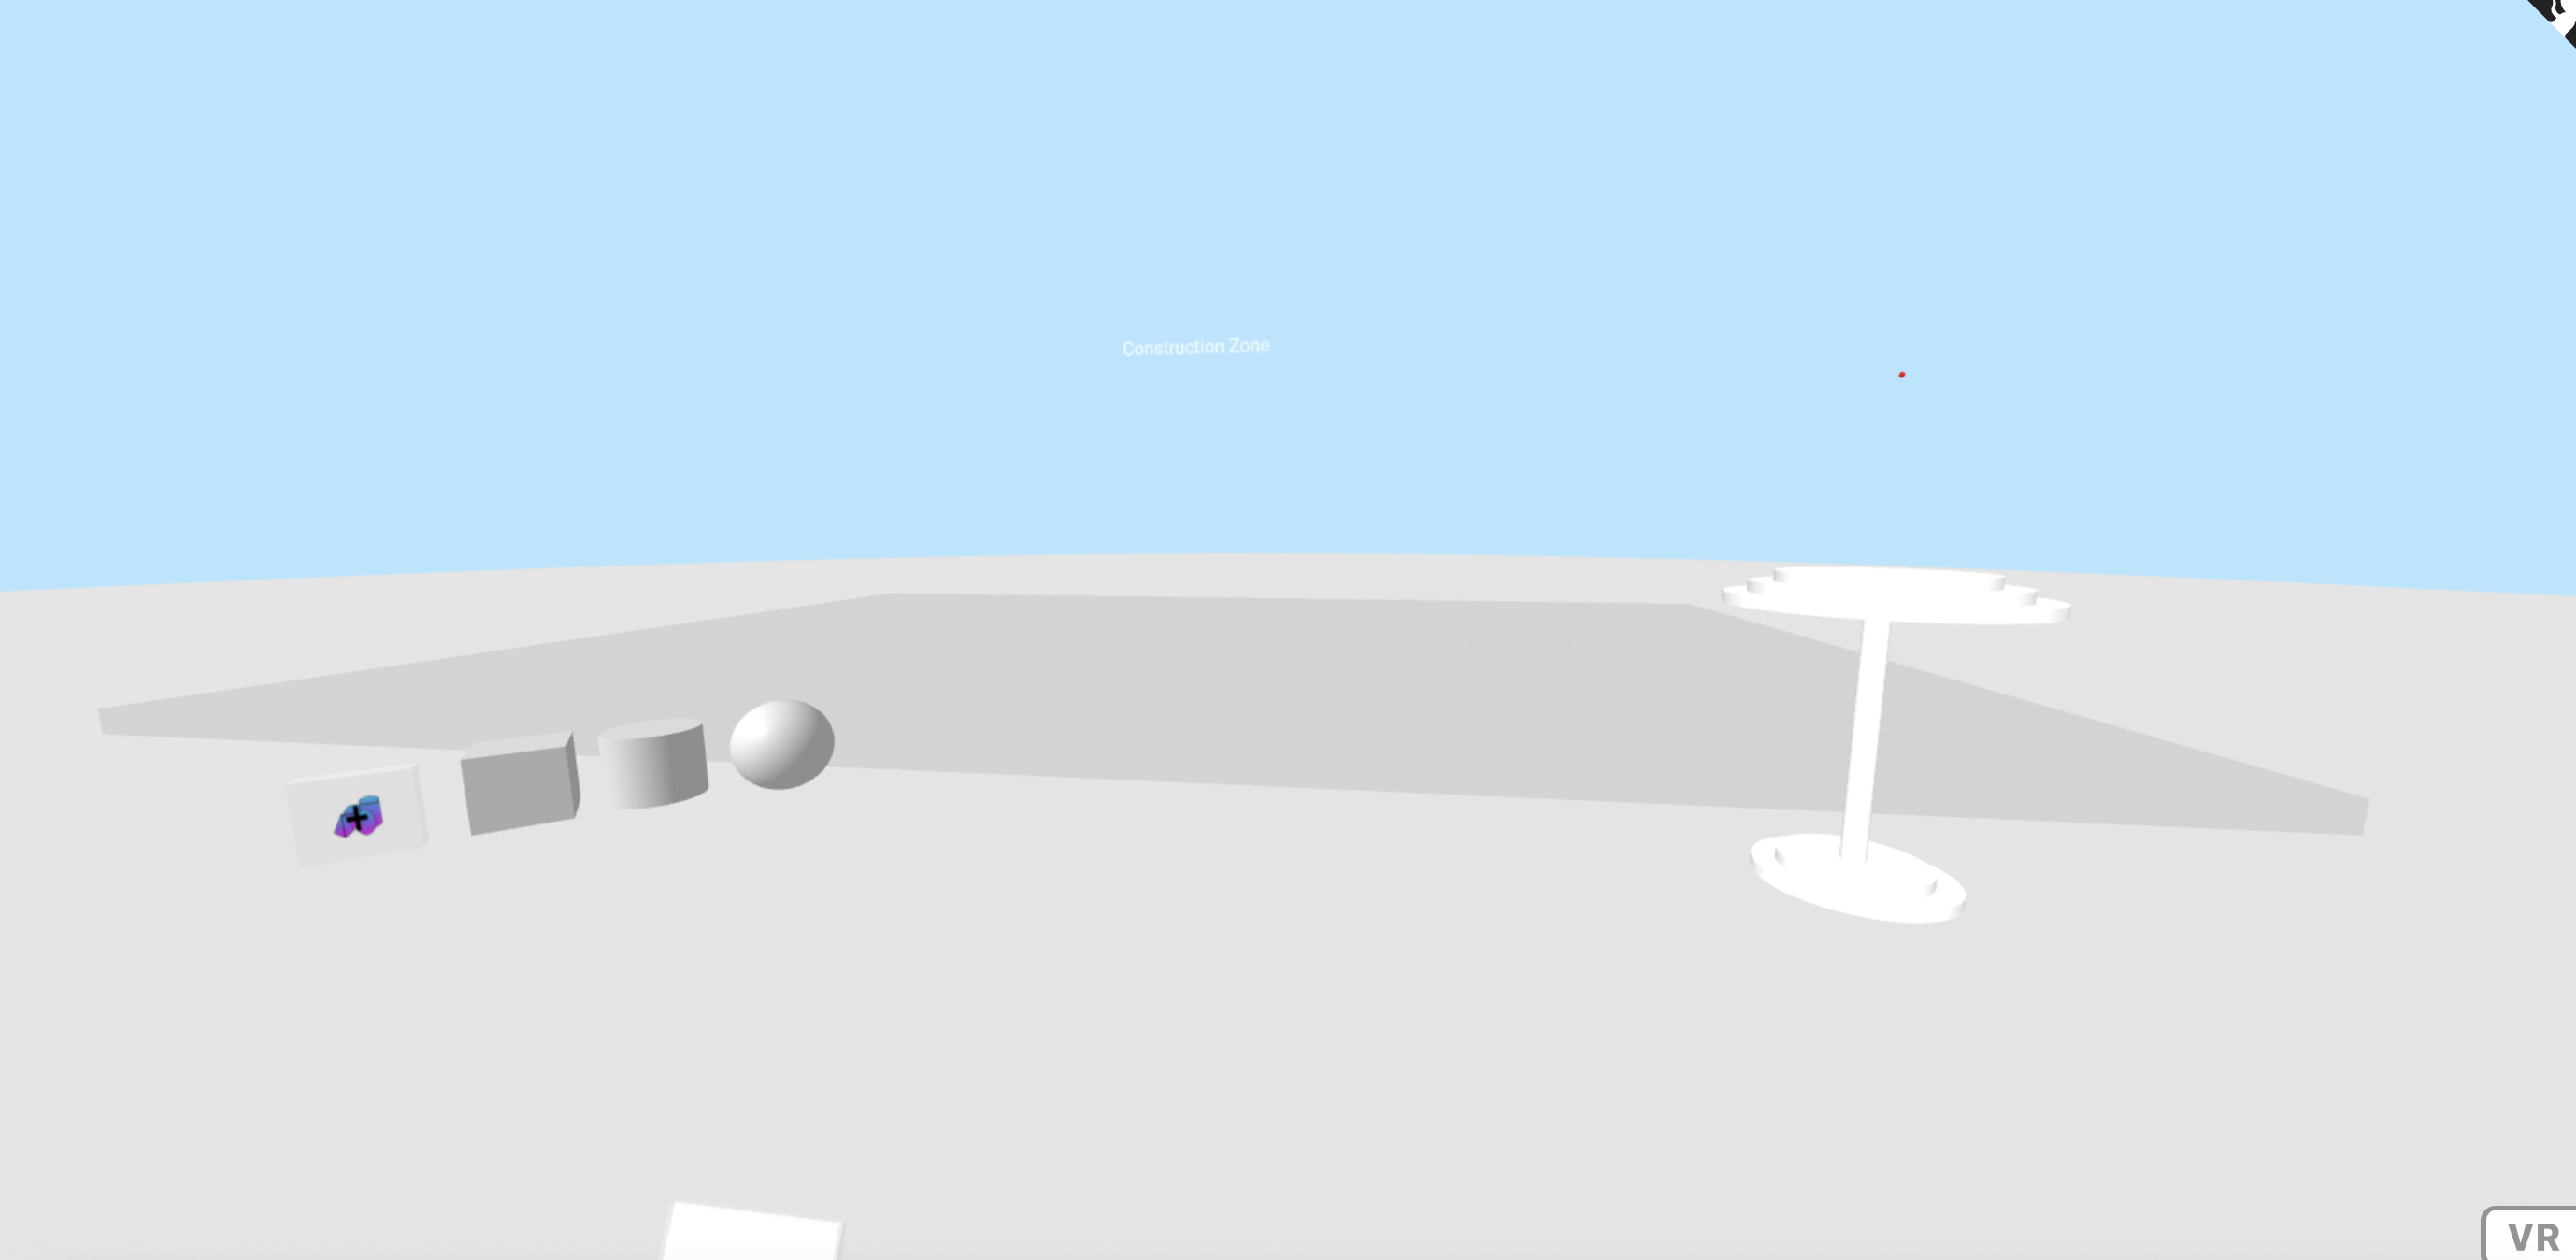
\includegraphics[width=9cm, keepaspectratio]{MemoriaTFG-JulianPerez/img/gen.png}
  \caption{Escenario general}\label{gen}
\end{figure}

Las figuras que sean clickables se verá mas claro que se pueden clickar.
\begin{figure}[H]
  \centering
  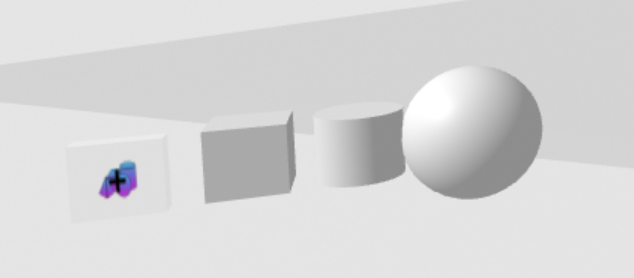
\includegraphics[width=7cm, keepaspectratio]{MemoriaTFG-JulianPerez/img/figs.png}
  \caption{Figura seleccionada}\label{scrum}
\end{figure}

Respecto al menú de creación de figuras y el modo grupo, haremos que sigan al usuario para se encuentre de una manera más accesible y escondida, de este modo, visualizar mejor el escenario. Respecto al menu de las figuras con ayuda de la creación de componentes, lo rediseñaremos para que se muestre de una manera más sencilla y vistosa y le añadiremos la posibilidad de poder esconderlo. También colocaremos de una manera mas adecuada el menú de modificación de la figura. 

\begin{figure}[H]
  \centering
  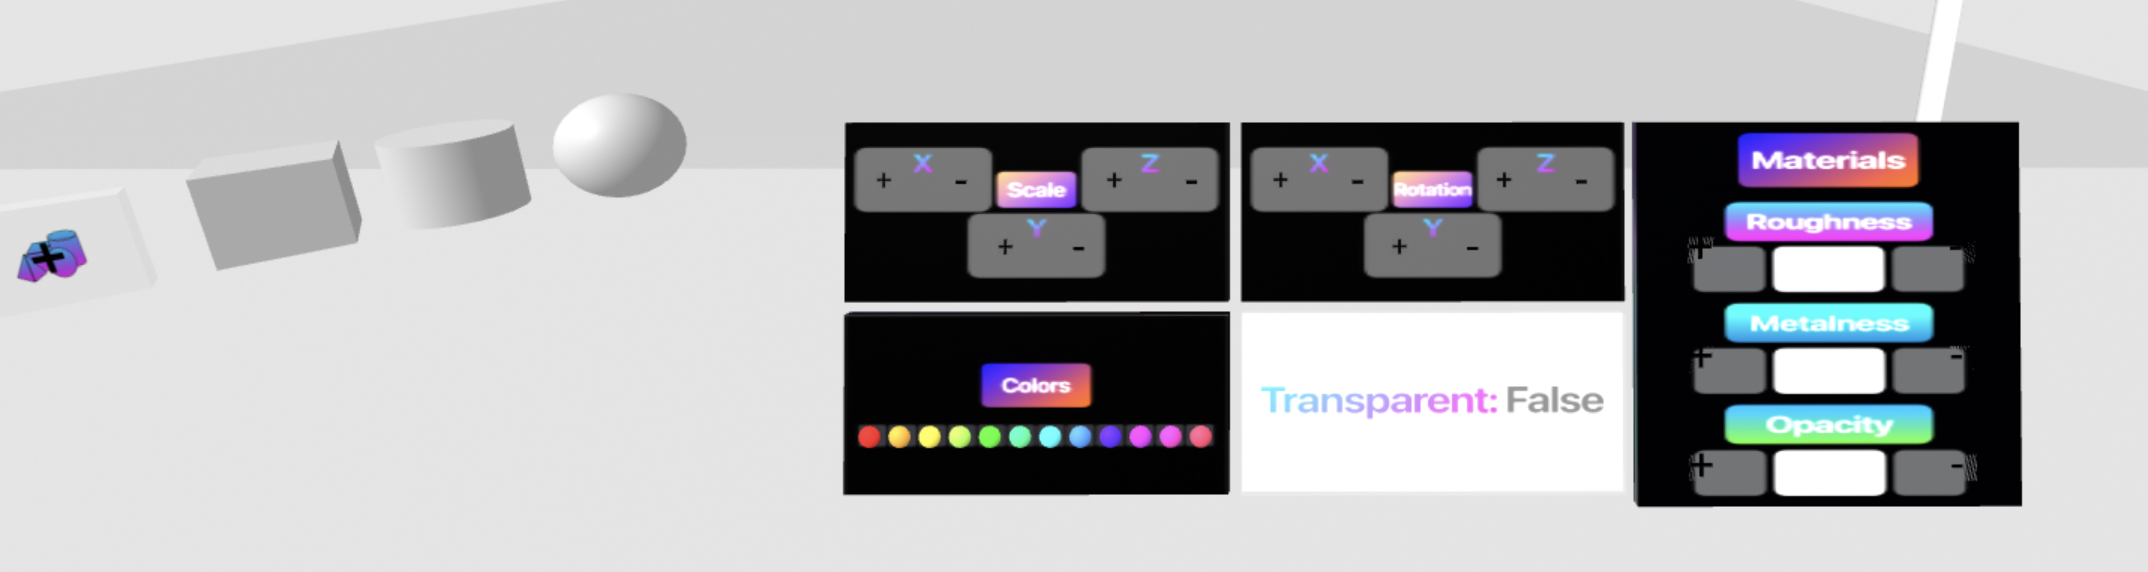
\includegraphics[width=10cm, keepaspectratio]{MemoriaTFG-JulianPerez/img/menu.png}
  \caption{Menú modificación figura}\label{scrum}
\end{figure}

Respecto al modo grupo cambiaré varias cosas, la primera, añadi una imagen al manejador para poder diferenciarlo de las otras figuras del escenario

\begin{figure}[H]
  \centering
  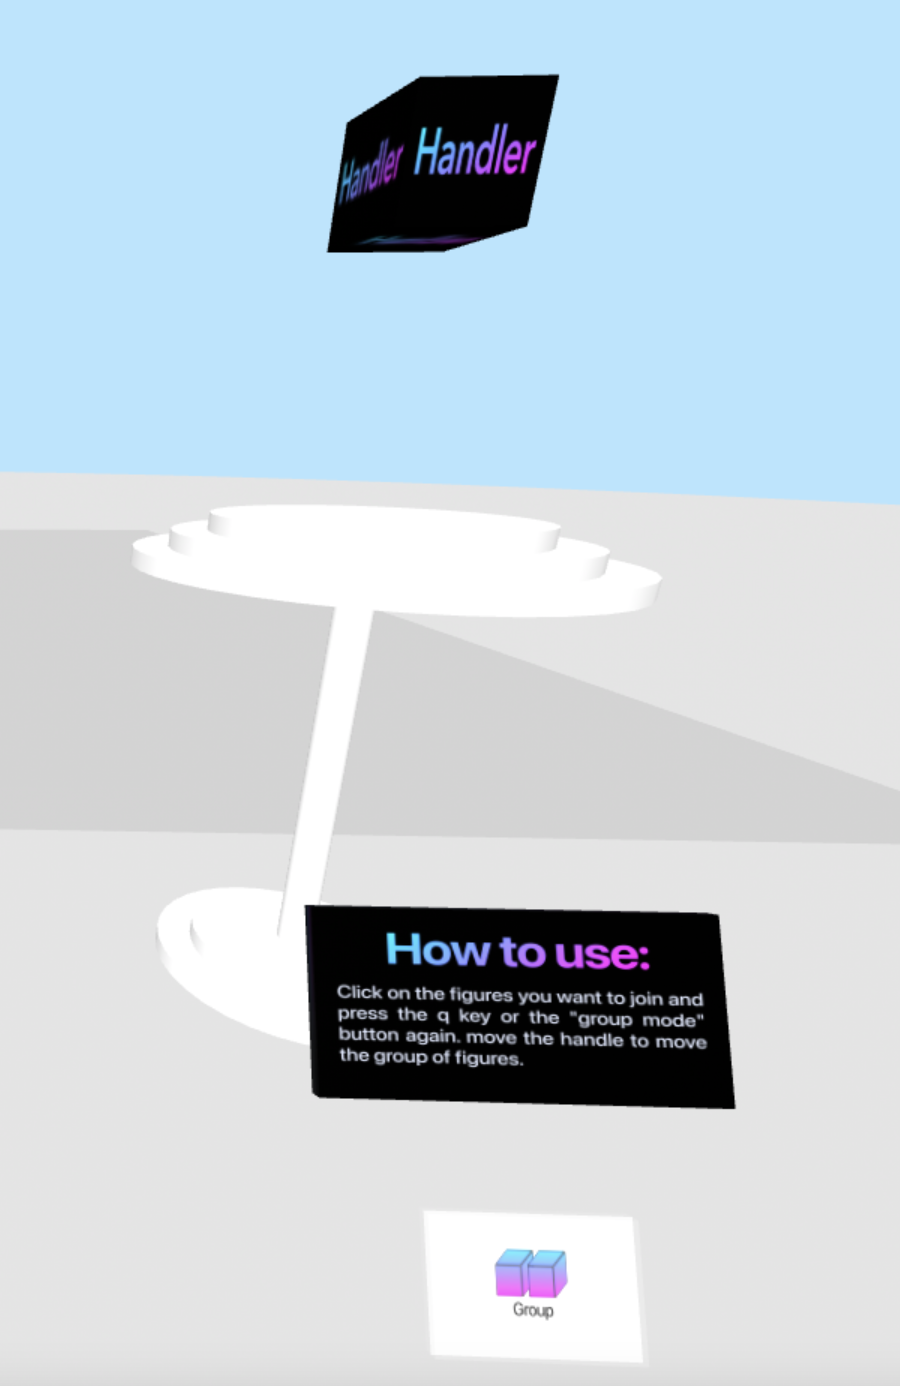
\includegraphics[width=4cm, keepaspectratio]{MemoriaTFG-JulianPerez/img/handler.png}
  \caption{Manejador}\label{scrum}
\end{figure}

y respecto a las figuras que selecciones para la creación del grupo, añadi, una animación para que el usuario sepa que figura ha seleccionado.


\textbf{Tarea 2}

En esta tarea, nos centraremos en añadir distintas figuras en 3D.

Crearé un menú para estas figuras en las cuales podremos elegir entre disitntas figuras las cuales están clasificadas por categorias. Para añadir estas figuras hemos utilizado el elemento \begin{verbatim} <a-asset-item>\end{verbatim} que nos facilita A-Frame.

El resultado lo podremos observar en el escenario de la manera que nos muestra la figura 3.18

\begin{figure}[H]
  \centering
  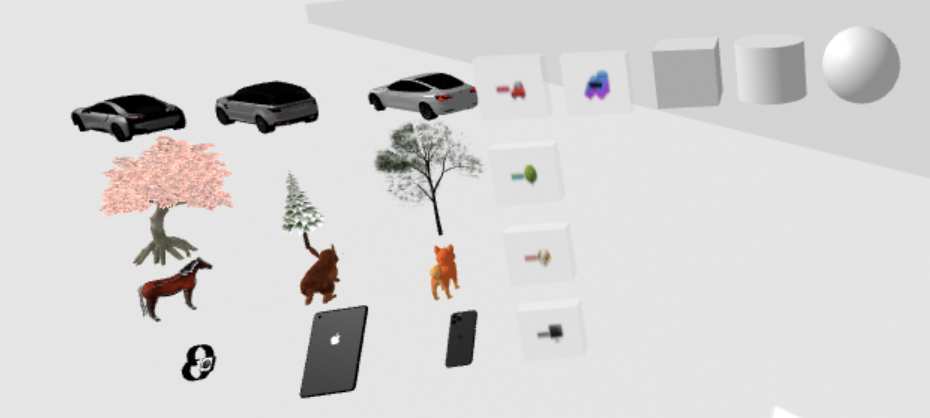
\includegraphics[width=12cm, keepaspectratio]{MemoriaTFG-JulianPerez/img/gltfs.png}
  \caption{Nuevas figuras del editor}\label{fig}
\end{figure}

\textbf{Tarea 3}

En esta tarea añadiremos nuevas formas de modificar mas propiedades de las figuras.

Con la creación de nuevos componentes añadi la capacidad de modificar la horientación de la figura en los tres ejes, rugosidad,la metalización y la opacidad a esta última se le añade una funcionalidad especial la cual puede hacer la figura transparente.

El resultado se puede observar en la figura 3.16

\textbf{Tarea 4}

Por últmo nos centraremos en la compatibilidad de nuestro escenario con la gafas de realidad virtual, en concreto, las Oculus Quest. 

\subsection{Resultado}

Como resultado de este sprint, puedo decir que estoy más cerca de la versión final. Solo nos quedaría refinar algunos aspectos. Hemos consguido crear nuevas funcionalidades, mejorar nuestra aplicación y hacerla mas usable para el usuairo. Este sprint está disponible en el repositorio del proyecto, tanto el codigo \footnote{\url{https://github.com/julianperezm/A-frame/tree/master/SeventhExercise}} como el escenario, ya sea la version escritorio \footnote{\url{https://julianperezm.github.io/A-frame/SeventhExercise/Desktop.html}} o la versión de realidad virtual \footnote{\url{https://julianperezm.github.io/A-frame/SeventhExercise/Glasses.html}}

\section{Sprint Final}
En este sprint nos centraremos en el final del proyecto puliendo los últimos detalles y añadiendo las ultimas funcionalidades de la aplicación.

\subsection{Objetivo}
Los objetivos de este sprint será seguir mejorarando la interfaz de usuario haciendolo mas intuitivo y añadir dos nuevas funcionalidades para mejorar el desarrollo del editor, nos centraremos en la inclusión de nuevos ambientes y seguiremos desarrollando las existentes.

\subsection{Desarrollo}
Seguiremos dividiendo las el desarrollo del sprint en tareas.

\textbf{Tarea 1}

En este tarea seguiremos mejorando la interfaz de usuario para hacerla más intutuita y sencilla para el usuario, añadiremos nuevos atributos, como son el procentaje de progeso de las modificaciones de los materiales que se les pueden realizar a las figuras 

\begin{figure}[H]
  \centering
  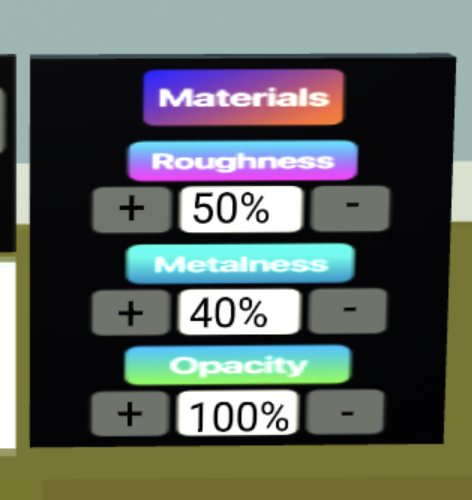
\includegraphics[width=6cm, keepaspectratio]{MemoriaTFG-JulianPerez/img/menu2.png}
  \caption{Nuevo menú de propiedades}\label{menu2}
\end{figure}

Tambien añadiremos una luz en el podium para que las modificaciones que le hacemos a la figura se puedan visualizar de una manera más clara

\begin{figure}[H]
  \centering
  \begin{minipage}[b]{0.4\textwidth}
 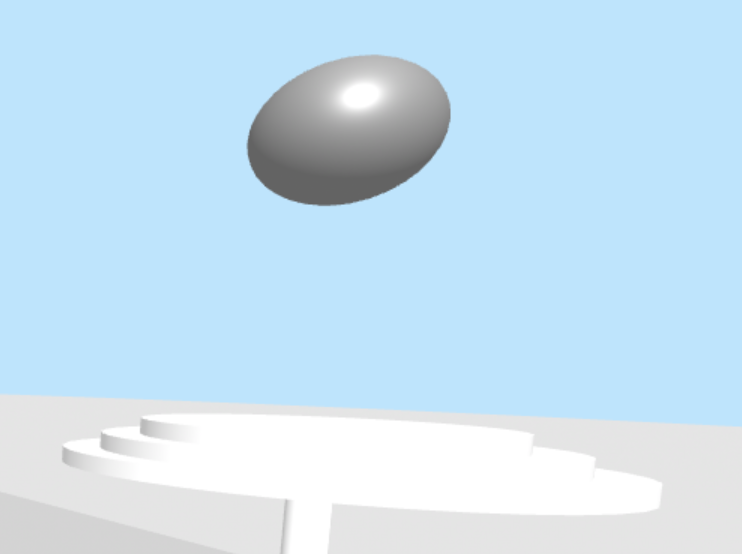
\includegraphics[width=7cm]{MemoriaTFG-JulianPerez/img/sinluz.png}
  \caption{Podium sin luz}\label{single}
  \end{minipage}
  \hfill
  \begin{minipage}[b]{0.4\textwidth}
  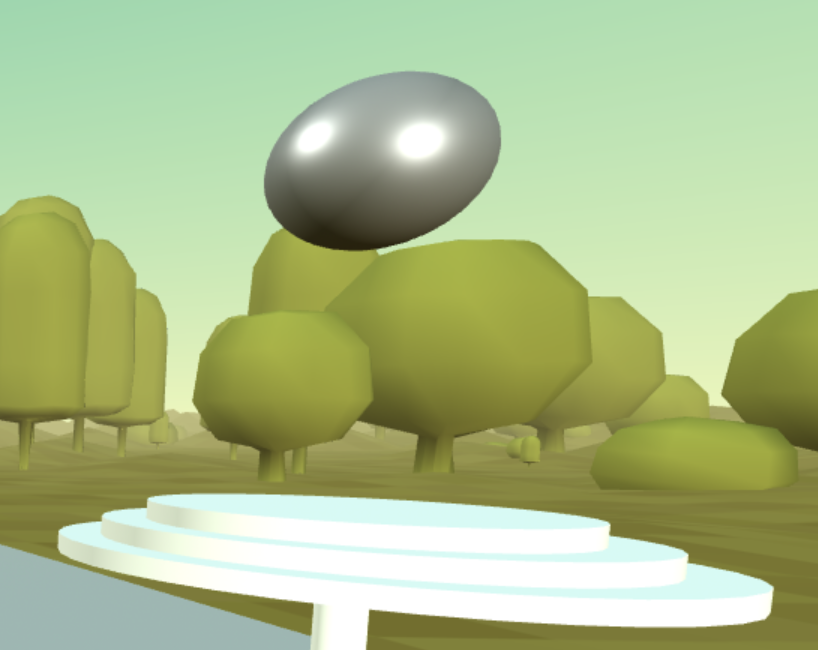
\includegraphics[width=7cm]{MemoriaTFG-JulianPerez/img/luz.png}
  \caption{Podium con luz}\label{scrum}
  \end{minipage}
\end{figure}

\textbf{Tarea 2}

En esta tarea nos centraremos en mejorar la funcionalidad de modo grupo, añadiremos un botón para así poder eleminar el manejador y el escenario quede mucho mas limpio.

Además de esta mejora añadiremos una funcionalidad la cual te permita cambiar de ambiente según le plazca 

La eliminación de los manejadores es posible añadiendo un componente que añada opacidad a dichas figuras. el escenario con manejadores quedaría como muestra la figura 3.22 y sin manejadores como la figura 3.23

\begin{figure}[H]
  \centering
  \begin{minipage}[b]{0.4\textwidth}
 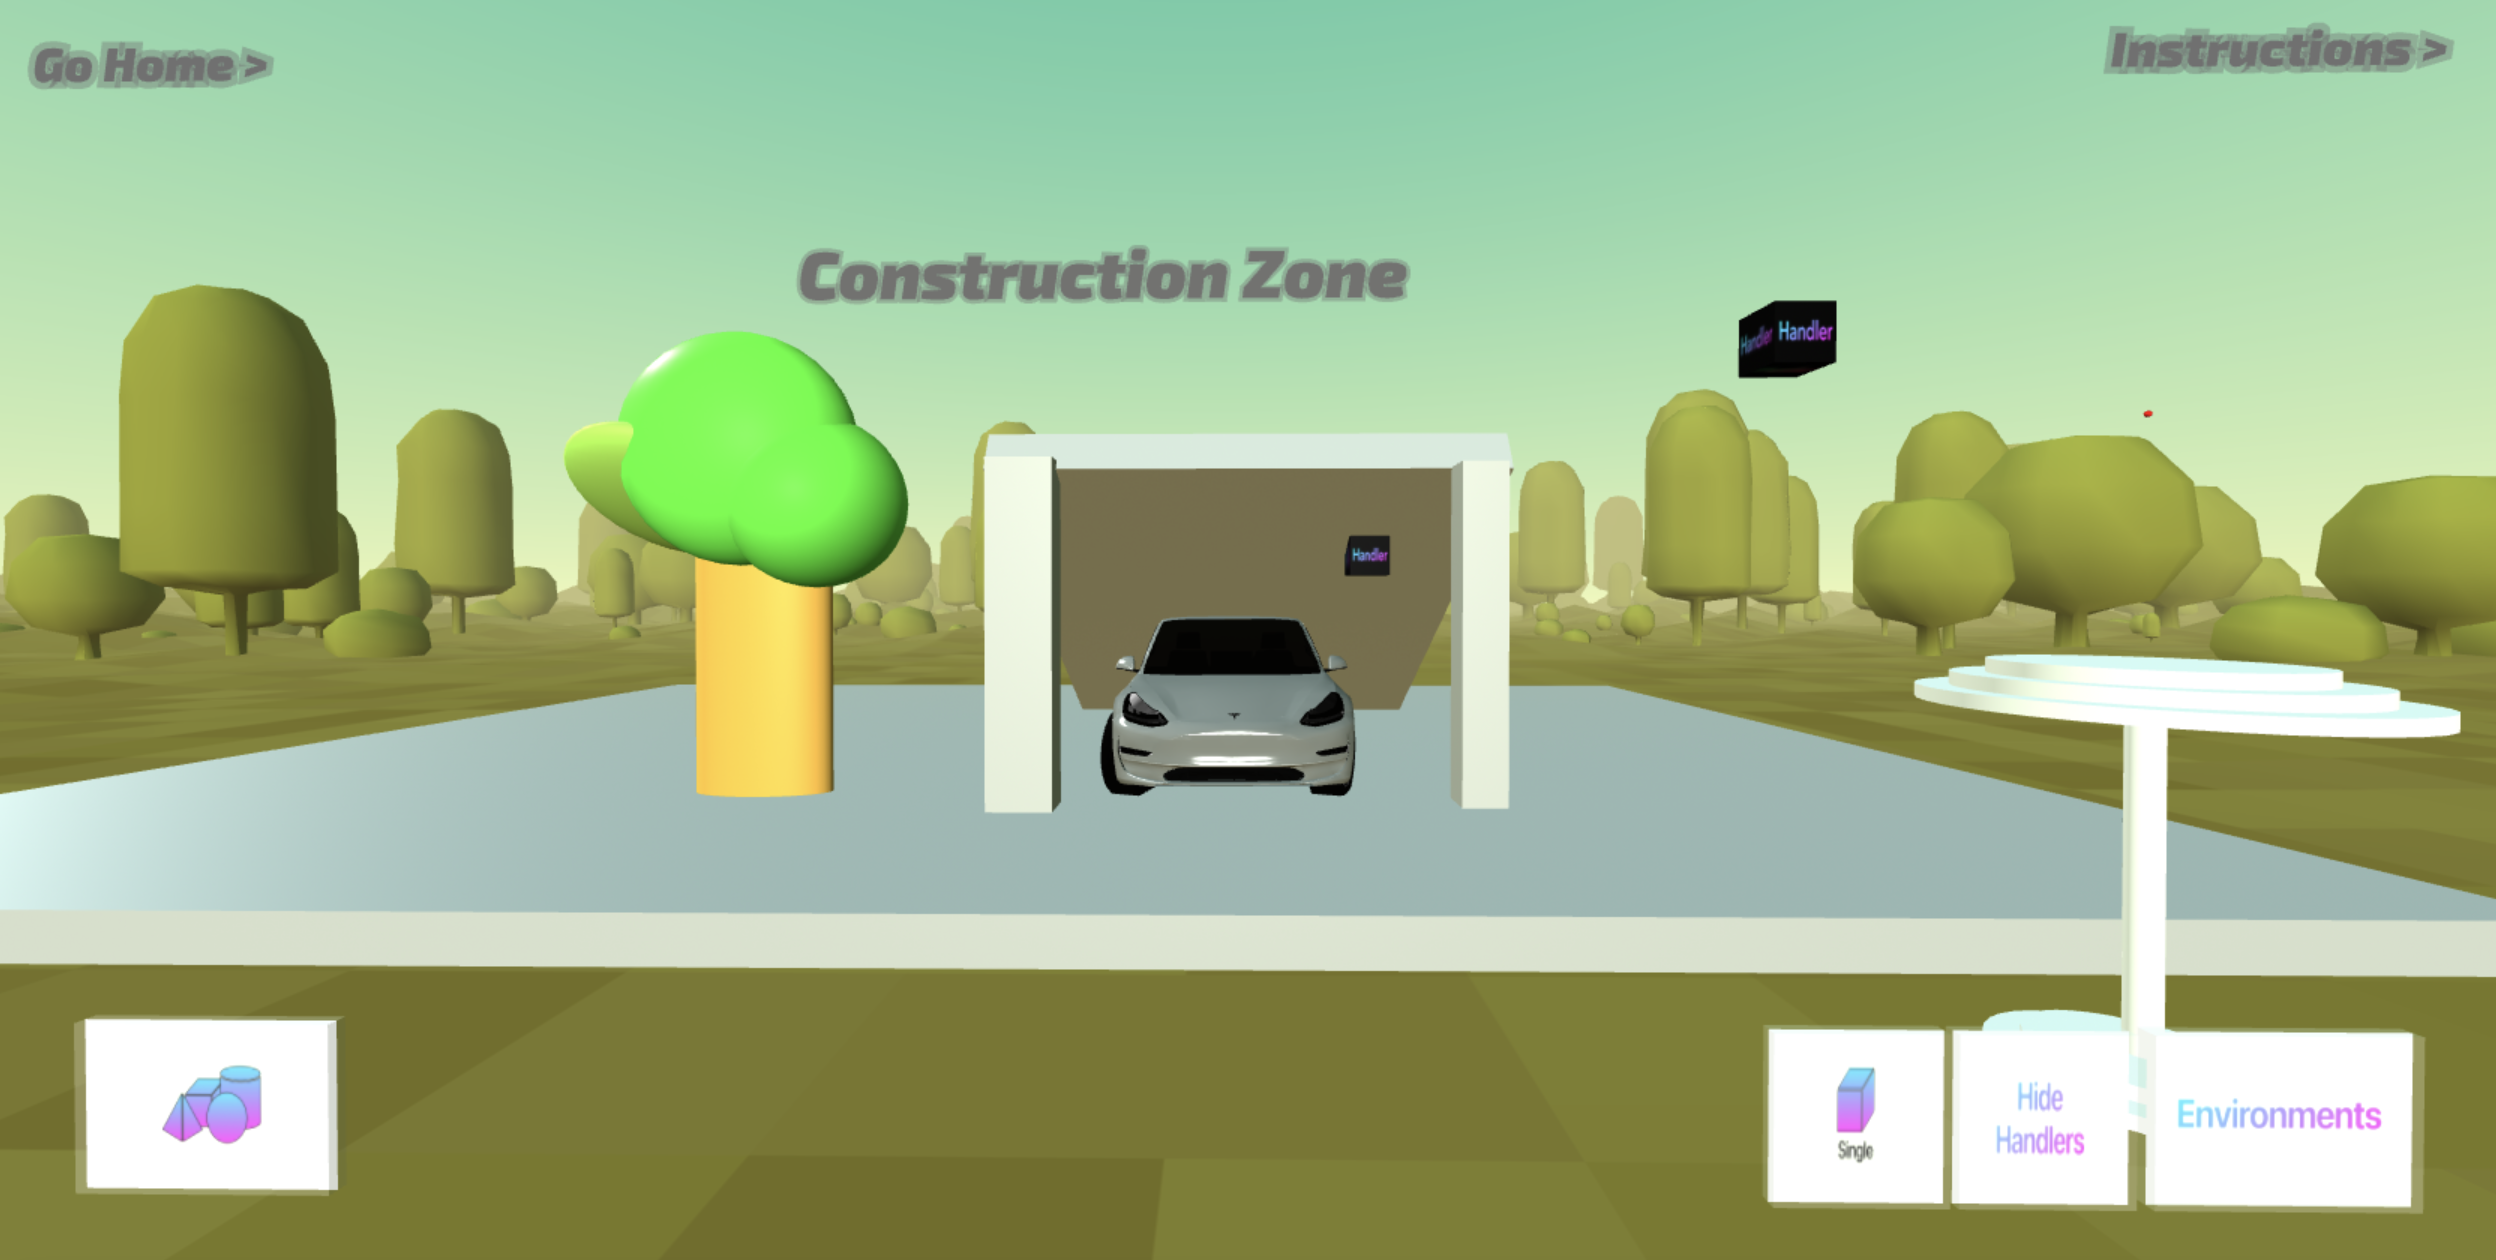
\includegraphics[width=7cm]{MemoriaTFG-JulianPerez/img/conm.png}
  \caption{Escenario con manejadores}\label{single}
  \end{minipage}
  \hfill
  \begin{minipage}[b]{0.4\textwidth}
  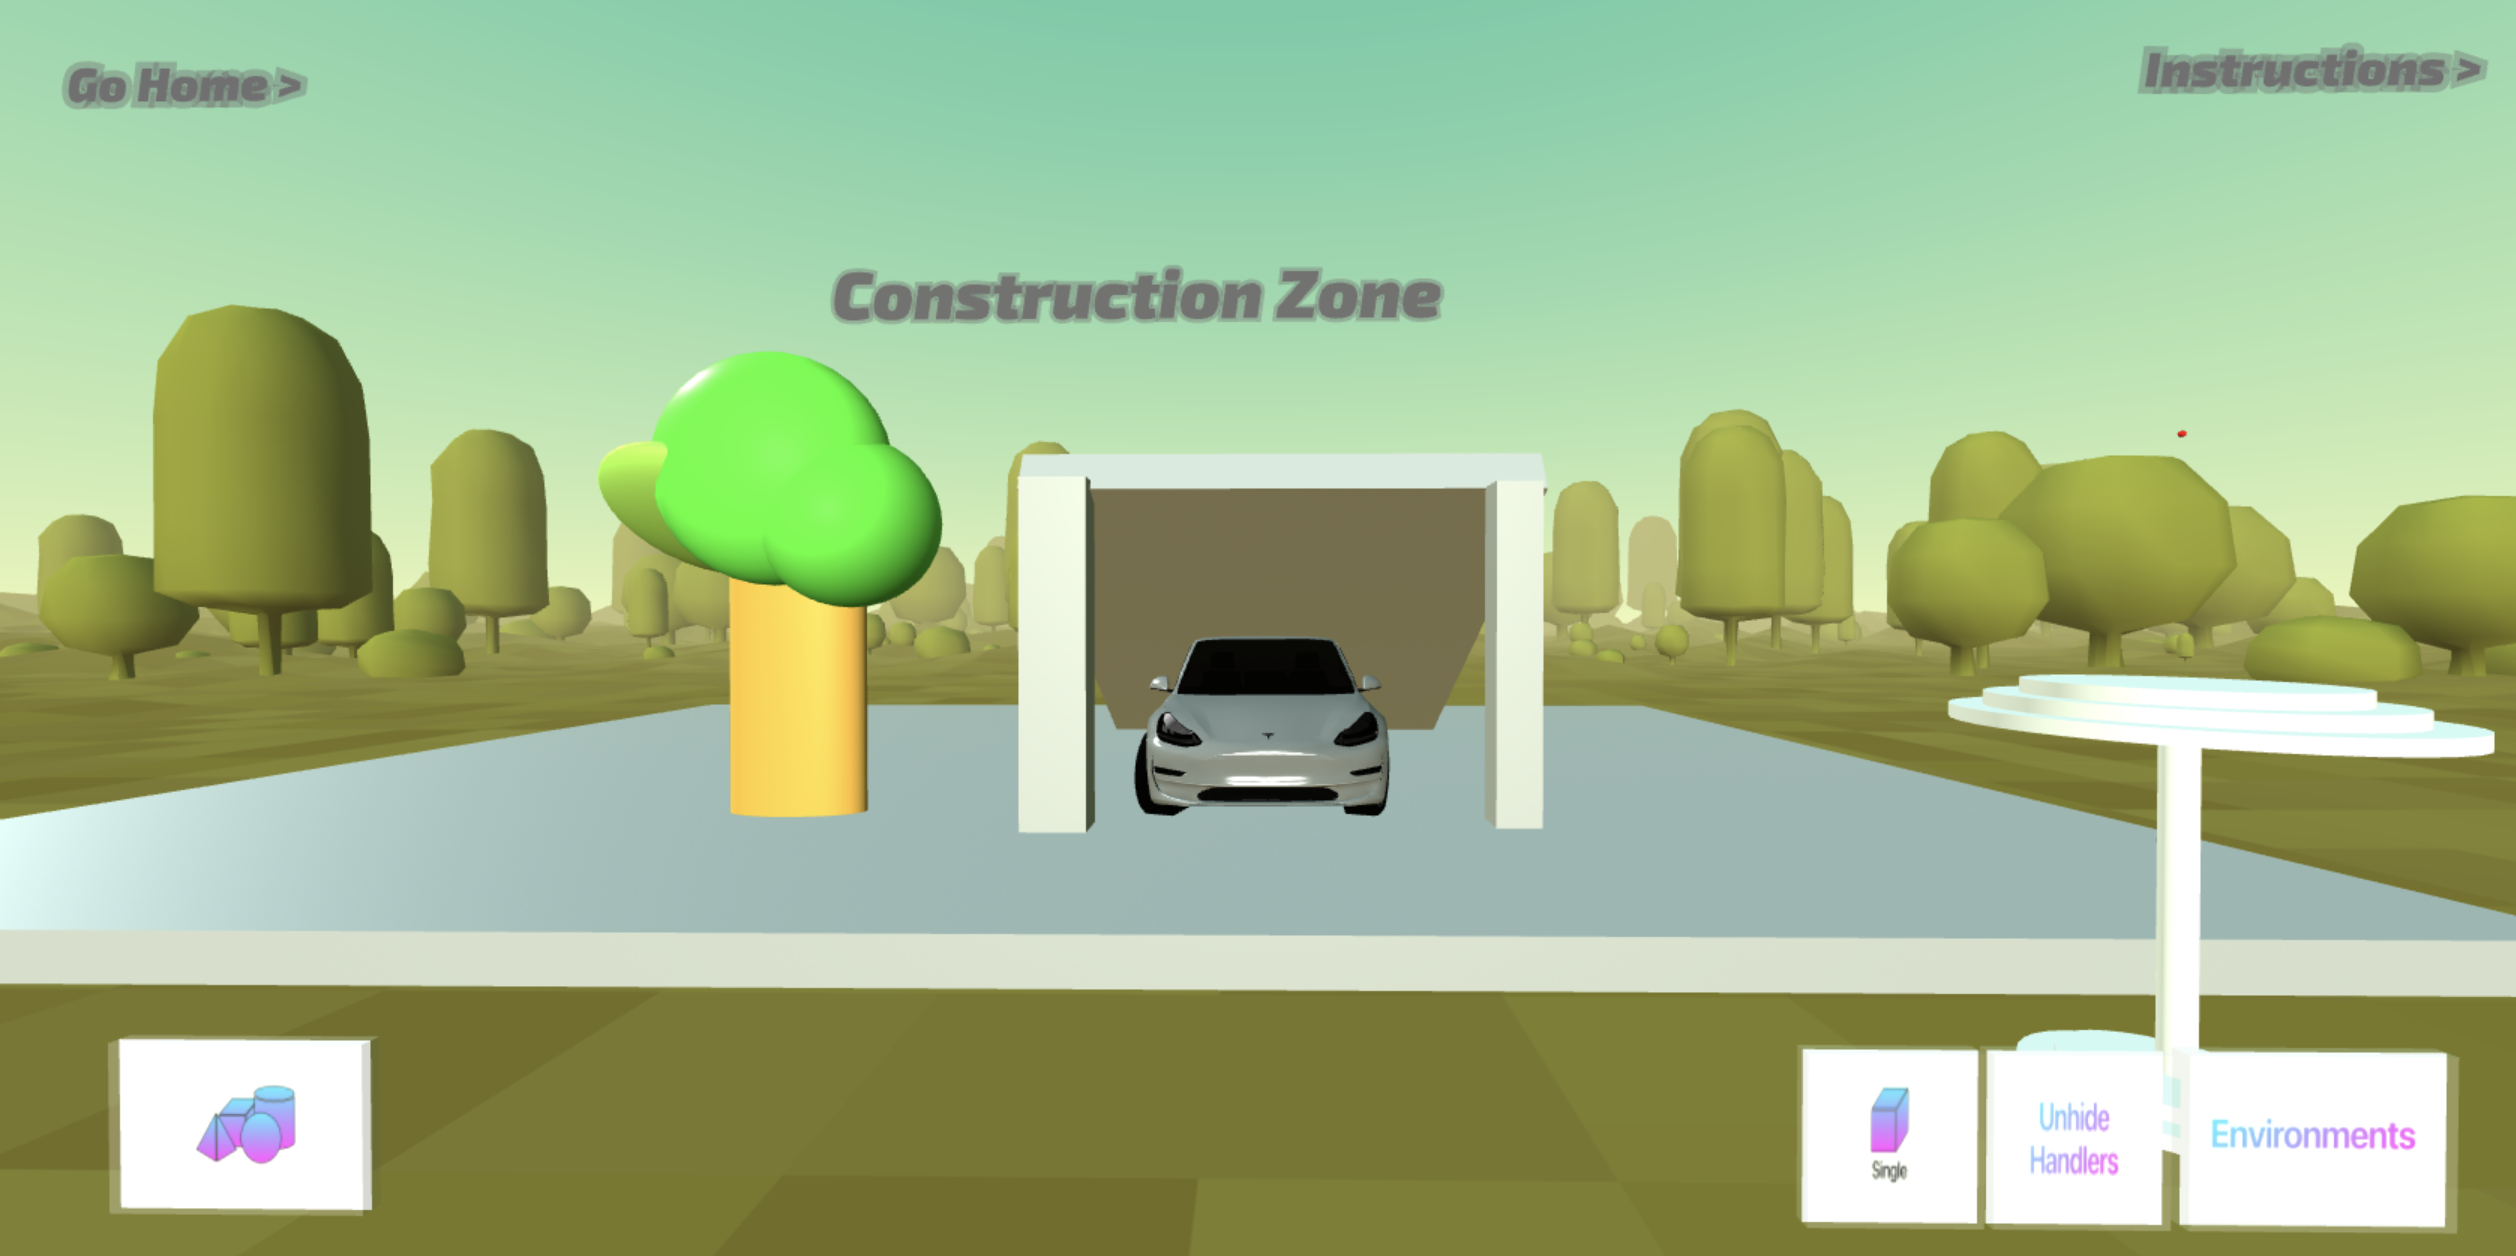
\includegraphics[width=7cm]{MemoriaTFG-JulianPerez/img/sinm.png}
  \caption{Escenario sin manejadores}\label{scrum}
  \end{minipage}
\end{figure}

Para los cambios de ambientes utilizaremos un componente creado por la comunidad, se puede encontrar en su repositorio de github \footnote{\url{https://github.com/supermedium/aframe-environment-component}}. 

El resultado de esta parte de la tarea se puede visualizar en la escena con un desplegable en el que puedes elegir que ambiente usar como se muestra en la figura 3.24

\begin{figure}[H]
  \centering
  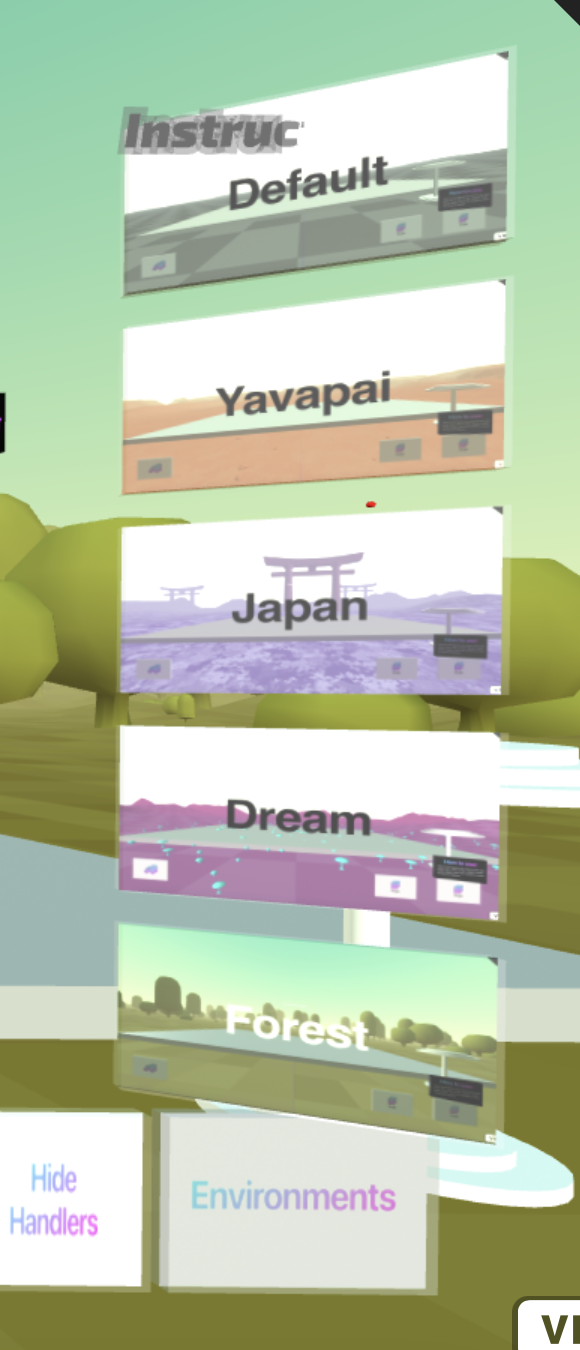
\includegraphics[width=4cm, keepaspectratio]{MemoriaTFG-JulianPerez/img/env.png}
  \caption{Menu de ambientes}\label{menu2}
\end{figure}

\textbf{Tarea 3}

Esta última tarea tratará de terminar la aplicación añadiendole una página principal

\begin{figure}[H]
  \centering
  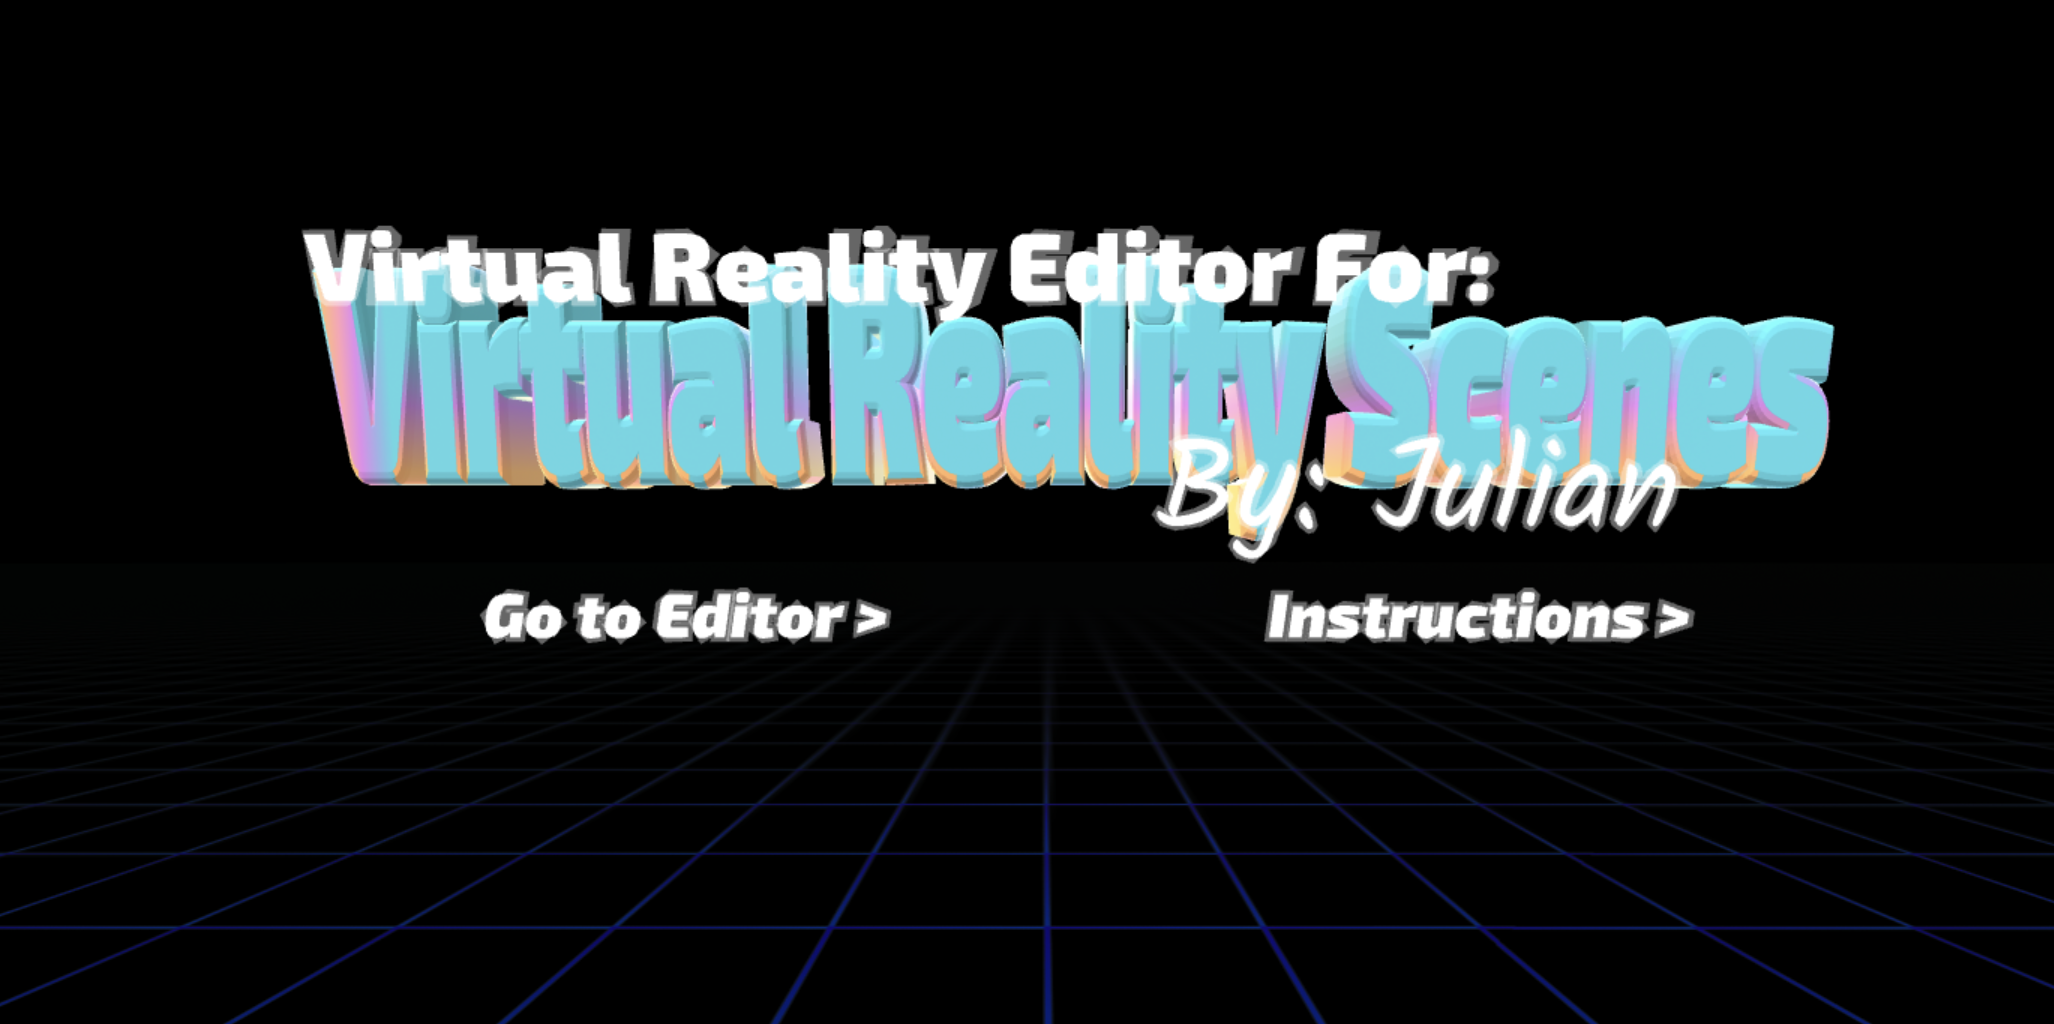
\includegraphics[width=10cm, keepaspectratio]{MemoriaTFG-JulianPerez/img/home.png}
  \caption{Página de inicio}\label{home}
\end{figure}

y otra página de instrucciones

\begin{figure}[H]
  \centering
  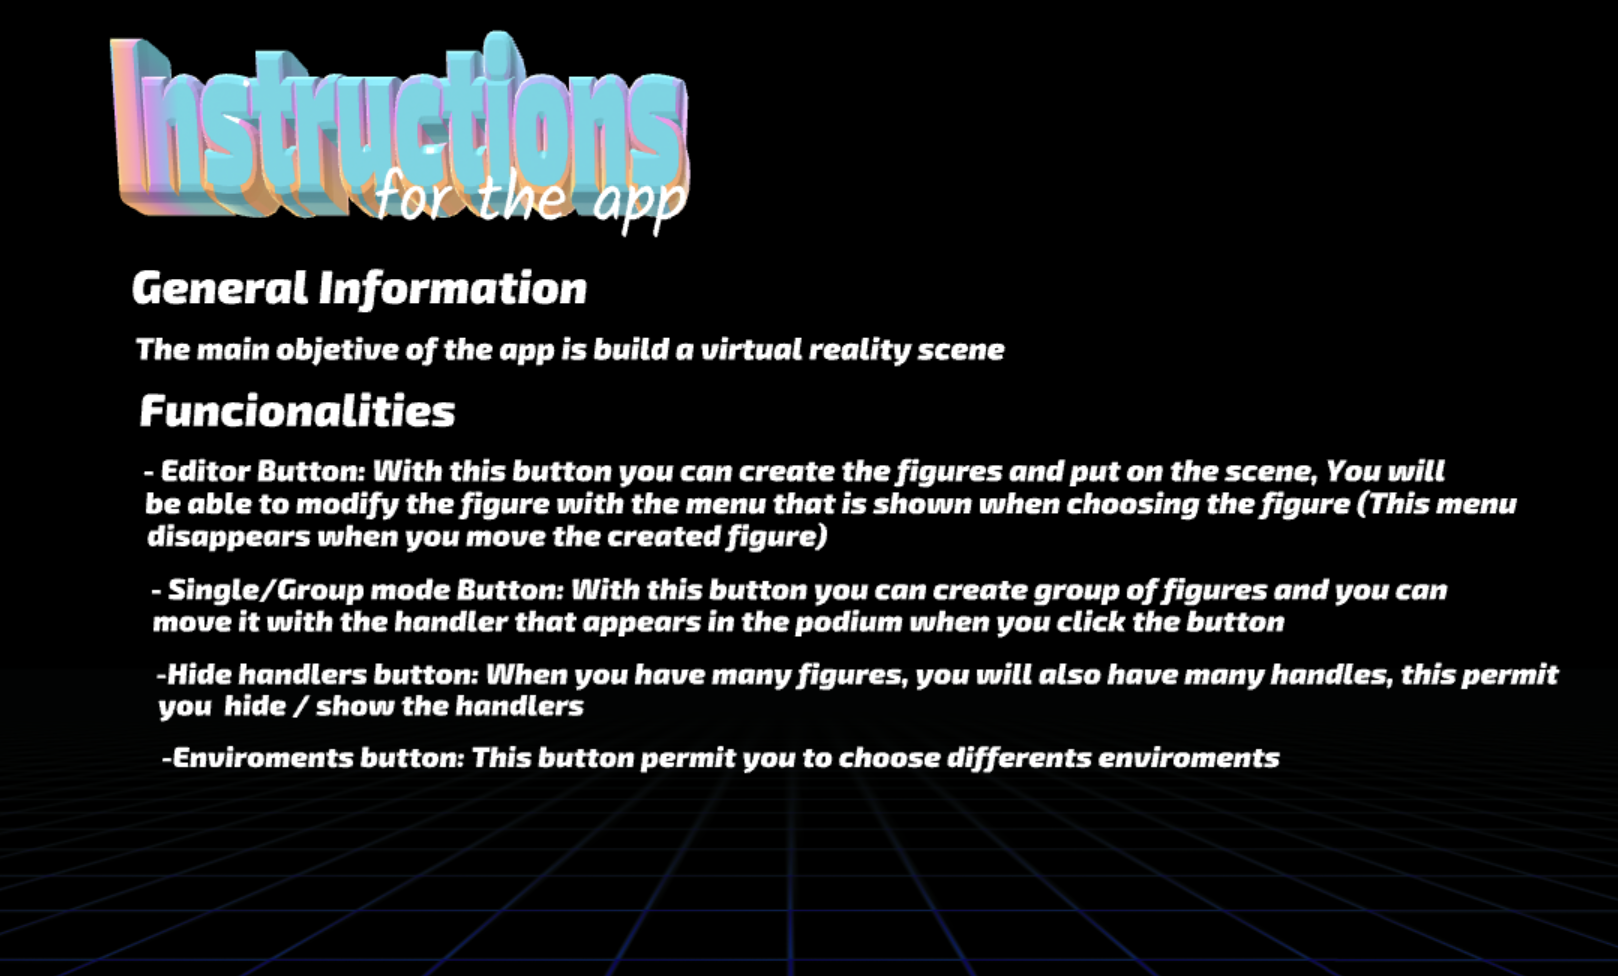
\includegraphics[width=10cm, keepaspectratio]{MemoriaTFG-JulianPerez/img/inst.png}
  \caption{Página de instrucciones}\label{home}
\end{figure}

Amabas son accesibles entre ellas ademas del escenario.

\subsection{Resultado}

En este utlimo sprint he conseguido terminar el proyecto, este proyecto puede seguir desarrollandose y mejorando, puede ser el comienzo de algo grande. El código \footnote{\url{https://github.com/julianperezm/A-frame/tree/master/Home}}.  y el escenario, ya sea la versión escritorio \footnote{\url{https://julianperezm.github.io/A-frame/Home/HomeDesktop.html}} o la versión compatible con las gafas \footnote{\url{https://julianperezm.github.io/A-frame/Home/HomeGlasses.html}} están disponibles en el repositorio del proyecto en GitHub.





\end{document}